\documentclass[letterpaper,journal]{IEEEtran}
\usepackage{amsmath,amsfonts,amssymb}
\usepackage{amsthm}
\usepackage{enumitem}
\theoremstyle{plain}
\newtheorem{theorem}{Theorem}
\newtheorem{lemma}{Lemma}
\theoremstyle{definition}
\newtheorem{assumption}{Assumption}
\theoremstyle{remark}
\newtheorem{remark}{Remark}
\newtheorem{problem}{Problem}
\usepackage{algorithmic}
\usepackage{algorithm}
\usepackage{array}
\usepackage[caption=false,font=footnotesize,labelfont=sf,textfont=sf]{subfig}
\usepackage{textcomp}
\usepackage{stfloats}
\usepackage{url}
\usepackage{verbatim}
\usepackage{graphicx}
\usepackage{placeins}
\usepackage{cite}
\hyphenation{op-tical net-works semi-conduc-tor IEEE-Xplore}

\begin{document}

\title{Distributed Orientation Control of Planar Formations in 3-D Space Using Angle and Bearing Constraints}

% IEEE Publication Technology,~\IEEEmembership{Staff,~IEEE,}

\author{Jianqing Li, Zhengyang Zhu}

% The paper headers
\markboth{Draft Manuscript}%
{Zhu: Distributed Formation Control for Four Agents in 3-D}

% \IEEEpubid{0000--0000/00\$00.00~\copyright~2021 IEEE}
% Remember, if you use this you must call \IEEEpubidadjcol in the second
% column for its text to clear the IEEEpubid mark.

\maketitle

\begin{abstract}
This paper addresses net-based aerial interception using four quadrotor unmanned aerial vehicles (QUAVs) to carry a capture net in three-dimensional (3-D) space. The objective is to keep the net spanned and oriented toward the incoming target during 3-D maneuvers. A distributed formation control scheme is proposed based on bearing and distance information. Angle constraints prescribe a four-agent square shape, while a single designated agent measures distances to regulate the formation scale. An explicit plane-normal control law orients the formation plane to face the target. A coplanarity control term using only local bearing measurements ensures that the net remains spanned throughout the interception. Each agent measures only the bearing information required by the control law in its own local coordinate frame. Only the distance-measuring agent communicates with its neighbors, and alignment of the agents' coordinate frames is not required. The necessity of the coplanarity constraint is confirmed by an ablation study, in which removing the term causes agents to drift out of plane. The overall scheme is further validated on a simplified QUAV model in a net-capture scenario with elastic cables, demonstrating its effectiveness.
\end{abstract}

\begin{IEEEkeywords}
Formation control, multi-agent systems, angle constraints, plane orientation, coplanarity control, net capture.
\end{IEEEkeywords}

\section{Introduction}
\IEEEPARstart{T}{he} rapid proliferation of small unmanned aerial vehicles (UAVs) has created an urgent demand for effective counter-UAS measures, as conventional air defense systems are ill-suited to intercept such small, slow, and low-altitude threats. In response, a broad range of counter-UAS measures has been investigated. Electromagnetic jamming and kinetic interception risk uncontrolled descent and collateral damage, while GPS spoofing and protocol attacks are ineffective against autonomous drones that navigate without external signals. Physical capture using a net carried by cooperative UAVs circumvents these limitations~\cite{rothe2019concept}. Among the formation geometries proposed for net-based interception are the four-UAV square configuration~\cite{tolman2017counter} and the three-UAV triangular configuration~\cite{chakravarthy2021interception,wang2022discrete}. Reliable interception requires the carrier UAVs to maintain a precise planar formation that keeps the net open and oriented toward the target, a problem that reduces to formation control in 3-D space.

Formation control methods can be categorized by the type of sensed and controlled variables they employ~\cite{oh2015survey}. Position-based approaches require each agent to know its absolute position with respect to a global coordinate system, which is often unavailable in GPS-denied environments~\cite{nguyen2020gps}. Displacement-based methods measure the relative positions of neighboring agents but require all agents to share a common sense of direction---that is, their local coordinate frames must be mutually aligned---which is difficult to guarantee under sensor noise and magnetic interference~\cite{demarina2021displacement}. Bearing-based methods rely on bearing rigidity theory to maintain relative directions between agents, but still require agents to know a global reference frame~\cite{trinh2016bearing}. Distance-based methods control inter-agent distances, which are independent of the orientation of each agent's coordinate frame. However, distance sensing requires dedicated ranging hardware that adds weight and power consumption to small aerial platforms. Angle-based methods use only angle measurements, which can be obtained from low-cost monocular cameras or direction-finding arrays without any coordinate frame alignment. Angle sensors are cheaper and more accessible than distance sensors~\cite{hu2023angle,gong2023review}. Owing to these advantages, angle-based formation control has attracted considerable research interest in recent years.

Angle constraints are invariant under translation, rotation, and scaling. To prescribe formation scale, angle--distance approaches that operate entirely in local coordinate frames without requiring frame alignment have been extensively studied in recent years~\cite{li2025localInfo,shao2024directed}. These works, however, assume that all agents lie in a common plane, an assumption that is difficult to guarantee in practice. Moreover, angle and distance constraints are inherently rotation-invariant and therefore cannot prescribe the orientation of the formation plane in 3-D space. For planar formations embedded in 3-D space, a few results address plane orientation control. Sun et al.~\cite{sun2017distributed} proposed a distance-based method that specifies the directions of two relative position vectors to fix the formation orientation, but it requires distance sensing on all edges and global coordinate frame alignment for the orientation agents. Li et al.~\cite{li2024circle} achieved circle formation on an arbitrary 3-D plane without distance measurements, yet the vertically take-off and land (VTOL) model employed therein restricts the formation plane to non-vertical orientations and the vehicles must encircle a fixed target point. Other 3-D formation orientation results rely on volumetric agent configurations. Chen et al. achieved rotation and scaling maneuvering of tetrahedral angle-rigid formations under a two-leader scheme~\cite{chen2022maneuvering}, and affine formation approaches control rotation as part of a full affine transformation via stress-matrix-based control~\cite{chen2020affine,xu2020affine}. These methods, however, require non-coplanar agent arrangements and degenerate when agents become coplanar, hence inapplicable to planar formation scenarios.

Motivated by the above considerations, this paper proposes a distributed formation control scheme for four agents forming a square in 3-D space. Each agent measures only the bearing information required by the control law in its own local coordinate frame, with one designated agent additionally measuring the distances to its two adjacent agents and communicating with them. Angle constraints prescribe the square shape and distance measurements regulate the formation scale, while an explicit plane-normal control law and a coplanarity term ensure the correct orientation and flatness of the formation plane during 3-D maneuvers. The main contributions of this paper are summarized as follows.
\begin{enumerate}[leftmargin=*,nosep]
\item A distributed plane-normal control scheme is proposed to align the formation plane with a prescribed target orientation. The scheme uses only bearing measurements from the agents involved in plane orientation, with the distance-measuring agent communicating with its neighbors, and drives the formation plane to face the incoming target direction.
\item A coplanarity control term that relies solely on local bearing measurements is introduced to keep the four agents on a common plane during 3-D maneuvers. Combined with the angle and distance constraints, this term keeps the net spanned throughout the interception process.
\item The formation control scheme is embedded into a simplified QUAV model with LESO-based disturbance compensation and demonstrated in a target-capture scenario with elastic cables, validating the integrated scheme under time-varying disturbances, parameter switches, and cable tension.
\end{enumerate}

%Motivated by the above discussion, this paper studies the distributed control problem of planar four-agent formations in 3-D space with prescribed orientation. Unlike volumetric formations, planar formations are intrinsically underconstrained in orientation: angle and distance constraints can determine the in-plane geometry, yet leave the formation-plane orientation unresolved. Moreover, planar formations are vulnerable to out-of-plane drift, since conventional angle constraints provide only weak sensitivity to coplanarity deviations.

%To address these challenges, this paper develops a distributed formation control framework that simultaneously regulates formation shape, scale, coplanarity, and plane orientation using only local bearing measurements and minimal distance sensing, without requiring global coordinate-frame alignment. The main contributions are summarized as follows:

%1.A distributed formation control framework is proposed for planar four-agent formations in 3-D space that simultaneously regulates formation shape, scale, and plane orientation using only local bearing measurements and minimal distance sensing, without requiring global coordinate-frame alignment.
%2.A coplanarity control mechanism is introduced to address the structural weakness of planar angle constraints under out-of-plane perturbations. It is shown analytically that conventional angle errors provide only second-order sensitivity to out-of-plane deviations, whereas the proposed coplanarity term restores first-order corrective behavior.
%3.The unique challenges of orientation regulation for planar formations in 3-D space are identified and addressed, including orientation underdetermination, normal-direction ambiguity, and coplanarity fragility. An undirected plane-normal formulation together with a hysteresis-based branch-selection mechanism is developed to ensure robust orientation regulation without singularity or chattering.

The remainder of this paper is organized as follows. Section~II formulates the formation control problem for four agents in 3-D space. Section~III presents the formation control design and its application to the net-capture scenario. Section~IV provides simulation results examining the performance of the proposed scheme.



\section{Problem Formulation}

Consider a group of four agents in space, with index set \(\mathcal V=\{1,2,3,4\}\).
The dynamics of agent \(i\) are described by the double integrator
\begin{equation}
\label{eq:agent-dynamics}
\dot p_i = v_i,\qquad
\dot v_i = u_i,
\qquad i\in\mathcal V,
\end{equation}
where \(p_i\in\mathbb R^3\) and \(v_i\in\mathbb R^3\) denote the position and velocity of agent \(i\) in a fixed global coordinate system, and \(u_i\in\mathbb R^3\) is the control input.

The in-plane square shape and scale are specified by angle and distance constraints as in~\cite{li2025localInfo}. The angle constraint set is
\begin{equation}
\label{eq:angle-set}
\mathcal A=\{(2,1,4),(3,2,1),(4,3,2),(1,4,3)\},
\end{equation}
with desired angles \(\alpha_{jik}^*=\pi/2\). The distance-constrained edges are \(\mathcal E_d=\{(1,2),(1,4)\}\) with desired length \(\ell^*>0\). The constraint set is illustrated in Fig.~\ref{fig:square_constraints}.

\begin{figure}[ht]
\centering

\includegraphics[width=\columnwidth,trim=12pt 12pt 12pt 12pt,clip]{figures/fig_1}
\caption{Target square with angle and distance constraints.}
\label{fig:square_constraints}
\end{figure}

For any two agents \(i\) and \(j\), let
\begin{equation}
q_{ij}=p_j-p_i,\qquad
d_{ij}=\|q_{ij}\|,
\end{equation}
denote the relative position vector and the inter-agent distance. The corresponding bearing vector is
\begin{equation}
\label{eq:bearing-definition}
b_{ij}=\frac{q_{ij}}{\|q_{ij}\|}.
\end{equation}
Since defining signed angles in 3-D requires additional reference directions or aligned coordinate frames, we adopt unsigned angles throughout \cite{chen2023angleRigidity3D}.
The interior angle formed by agents \(j\), \(i\), and \(k\) can then be computed from the bearing measurements as
\begin{equation}
\label{eq:angle-definition}
\alpha_{jik}=\arccos\left(b_{ij}^{T}b_{ik}\right),
\qquad \alpha_{jik}\in[0,\pi].
\end{equation}

To realize the above constraints, the following assumptions are made.

\begin{assumption}
Each agent is equipped with LOS sensing to acquire the relative direction information required by the formation controller.
\end{assumption}

\begin{assumption}
The initial positions of the agents are sufficiently close to a desired square formation, and are non-collinear.
\end{assumption}

\begin{assumption}
Only agent~\#1 is equipped with a distance sensor and can measure the distances to its neighboring agents; the other agents do not require distance-measuring capability.
\end{assumption}

Although the angle and distance constraints together specify the in-plane square shape and scale, they are invariant under rigid rotations in 3-D. Specifically, for any \(Q\in SO(3)\) and \(c\in\mathbb R^3\), the transformed positions \(\tilde p_i=Qp_i+c\) preserve all constrained distances and angles, i.e., \(\tilde d_{ij}=d_{ij}\) and \(\tilde\alpha_{jik}=\alpha_{jik}\), while the orientation of the formation plane changes accordingly. Hence the same square shape and scale admit a continuum of spatial orientations, and an additional plane-normal constraint is required to select the desired formation plane.

To describe the plane orientation, we define the unit normal vector of the plane spanned by agents \(i\), \(j\), and \(k\) as
\begin{equation}
\label{eq:general-normal}
N_{ijk}=b_{ij}\times b_{ik},\qquad
n_{ijk}=\frac{N_{ijk}}{\|N_{ijk}\|},
\end{equation}
which is well-defined whenever \(b_{ij}\) and \(b_{ik}\) are not collinear. The reference plane of the formation is taken as the plane spanned by agents~\#1, \#2, and~\#4, with normal \(n_{124}\) computed from~\eqref{eq:general-normal}.

Let \(n_d\in\mathbb R^3\), \(\|n_d\|=1\), be the prescribed target plane normal. For the capture net application, \(n_d\) and \(-n_d\) represent the same physical net opening orientation, as shown in Fig.~\ref{fig:orientation_branch}; the target set is therefore \(\mathcal N_d=\{n_d,-n_d\}\).

A natural error candidate is the cross product \(n_{124}\times n_d\). This quantity vanishes whenever \(n_{124}\) is parallel to \(n_d\), i.e., at both \(n_{124}=n_d\) and \(n_{124}=-n_d\). However, the raw error is antisymmetric under \(n_{124}\to -n_{124}\): it takes opposite signs at the two equivalent target branches. Since any restoring torque must be aligned with the error direction, the same control law would produce an attractive torque near \(+n_d\) and a repelling torque near \(-n_d\), driving formations from the \(-n_d\) branch toward \(+n_d\).

\begin{figure}[ht]
\centering
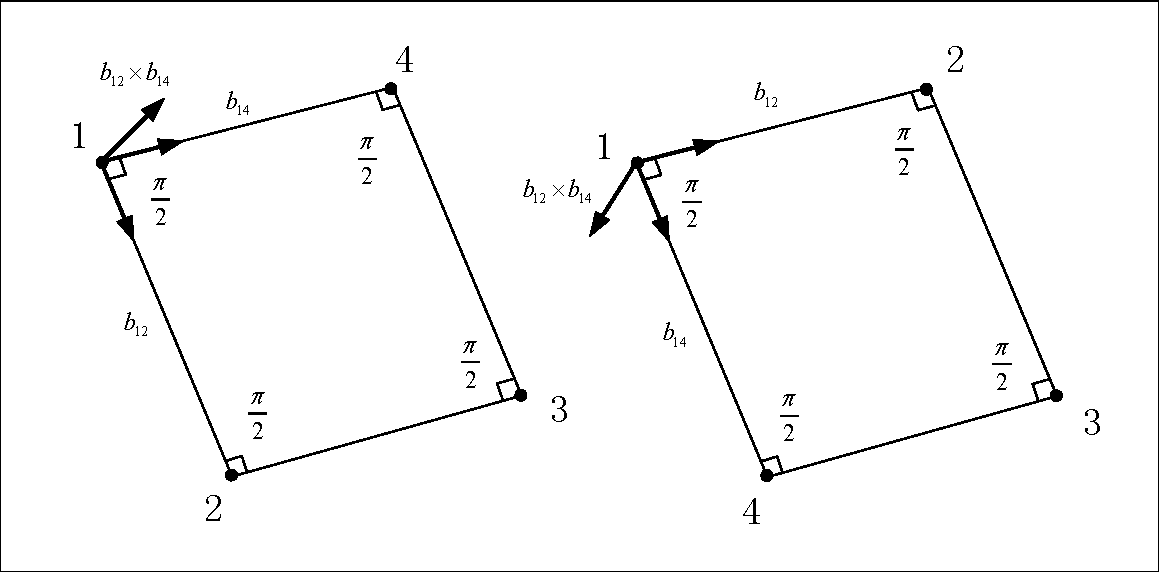
\includegraphics[width=\columnwidth,trim=2pt 2pt 2pt 2pt,clip]{figures/fig_2}
\caption{Both \(\pm n_d\) satisfy the undirected normal constraint, corresponding to two orientation branches.}
\label{fig:orientation_branch}
\end{figure}

To make both branches attractive while avoiding chattering near perpendicular configurations, a hysteresis-based branch selection is adopted. Define the scalar projection
\begin{equation}
c=n_{124}^{T}n_d,
\label{eq:projection-c}
\end{equation}
and let \(s_k\in\{+1,-1\}\) be a discrete switching state with a deadzone threshold \(\delta>0\). The branch selection rule is
\begin{equation}
\label{eq:branch-hysteresis}
s_k=
\begin{cases}
+1, & c > \delta,\\[2pt]
-1, & c < -\delta,\\[2pt]
s_{k-1}, & |c|\le\delta.
\end{cases}
\end{equation}
The selected target normal and the normal-direction error are then
\begin{equation}
\label{eq:normal-error}
\bar n_d = s_k n_d,\qquad
e_n = n_{124}\times \bar n_d.
\end{equation}
When \(|c|>\delta\), the branch closer to \(n_{124}\) is selected. When \(|c|\le\delta\), the formation plane is nearly perpendicular to the target plane, and \(s_k\) retains its previous value, preventing controller oscillation from noise-induced sign flips. This deadzone hysteresis renders both \(n_{124}=n_d\) and \(n_{124}=-n_d\) stable equilibria of the closed-loop system.

In 3-D maneuvering, the four agents may drift out of the reference plane. To ensure coplanarity, we require agent~\#3 to lie on the reference plane \(\{1,2,4\}\). The coplanarity error is defined as
\begin{equation}
\label{eq:coplanar-error}
e_{\mathrm{cop}}=b_{31}^{T}n_{234},
\end{equation}
where \(n_{234}\) is the unit normal of plane \(\{2,3,4\}\). Geometrically, \(|e_{\mathrm{cop}}|\) is proportional to the volume of the tetrahedron formed by the four agents and vanishes if and only if agent~\#3 lies on the reference plane. Agent~\#3 evaluates this error from the three local bearings \(b_{31}\), \(b_{32}\), and \(b_{34}\), as illustrated in Fig.~\ref{fig:coplanar_constraint}.

\begin{figure}[ht]
\centering
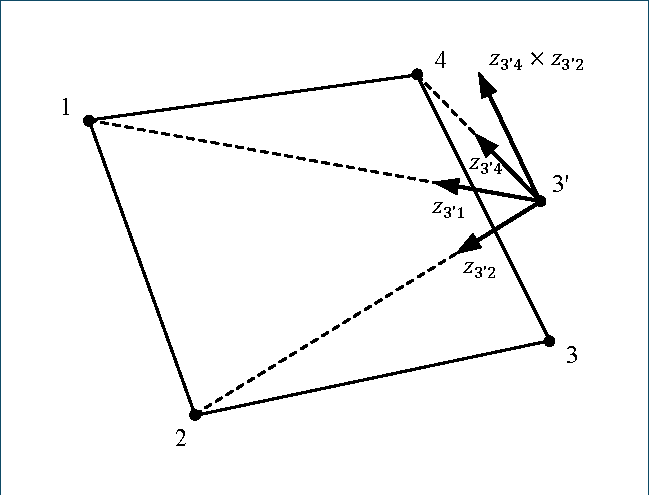
\includegraphics[width=\columnwidth,trim=12pt 12pt 12pt 12pt,clip]{figures/fig_3}
\caption{Coplanarity measurement via three local bearings.}
\label{fig:coplanar_constraint}
\end{figure}

Although the angle constraints guarantee coplanarity at the target configuration, they are relatively insensitive to out-of-plane perturbations, as the following analysis shows.

\begin{remark}
\label{rem:coplanarity-sensitivity}
The coplanarity error and the angle errors respond differently to out-of-plane deviations. Consider the target square
\[
\begin{aligned}
p_1^*&=[0,\ell^*,0]^{T}, &\quad p_2^*&=[0,0,0]^{T},\\
p_3^*&=[\ell^*,0,0]^{T}, &\quad p_4^*&=[\ell^*,\ell^*,0]^{T},
\end{aligned}
\]
and perturb \(p_3\) to \([\ell^*,0,h]^{T}\) while holding the other three agents fixed. A direct calculation yields \(e_{\theta_1}=e_{\theta_2}=e_{\theta_4}=0\) and
\[
\cos\theta_3=\frac{h^2}{(\ell^*)^2+h^2},
\]
hence \(e_{\theta_3}=-\frac{h^2}{(\ell^*)^2}+O(h^4)\), while
\[
e_{\mathrm{cop}}=-\frac{1}{\sqrt{2}\,\ell^*}h+O(h^3).
\]
Thus angle errors are only second-order sensitive to out-of-plane displacements, whereas the coplanarity error provides a first-order response. This structural insensitivity explains why angle-based terms alone cannot effectively restore coplanarity, making the coplanarity constraint necessary.
\end{remark}

Combining the above constraints, the desired formation set is
\begin{equation}
\label{eq:desired-formation-set}
\mathcal S(\ell^*,n_d)=\left\{
p\in\mathbb R^{12}\;\middle|\;
\begin{aligned}
&\alpha_{jik}=\alpha_{jik}^*, &&(j,i,k)\in\mathcal A,\\
&d_{ij}=d_{ij}^*, &&(i,j)\in\mathcal E_d,\\
&e_{\mathrm{cop}}=0,\; e_n=0
\end{aligned}\right\}.
\end{equation}

With the above setup, the formation control problem is stated as follows.

\begin{problem}
Consider the four-agent system \eqref{eq:agent-dynamics} under Assumptions~1--3. Design a distributed formation controller such that the closed-loop system achieves
\begin{align}
\lim_{t\to+\infty}
\bigl(\alpha_{jik}(t)-\alpha_{jik}^*\bigr)&=0,
& (j,i,k)&\in\mathcal A, \label{eq:angle-convergence}\\
\lim_{t\to+\infty}
\bigl(d_{ij}(t)-d_{ij}^*\bigr)&=0,
& (i,j)&\in\mathcal E_d, \label{eq:distance-convergence}\\
\lim_{t\to+\infty}e_{\mathrm{cop}}(t)&=0, \label{eq:coplanar-convergence}\\
\lim_{t\to+\infty}\|e_n(t)\|&=0, \label{eq:normal-convergence}\\
\lim_{t\to+\infty}
\bigl(v_i(t)-v_c^*(t)\bigr)&=0,
& i&\in\mathcal V. \label{eq:velocity-convergence}
\end{align}
Equations \eqref{eq:angle-convergence}--\eqref{eq:coplanar-convergence} together with \eqref{eq:normal-convergence} imply convergence to \(\mathcal S(\ell^*,n_d)\), while \eqref{eq:velocity-convergence} ensures velocity tracking.
\end{problem}


% \section{Where to Get \LaTeX \ Help --- User Groups}
\section{Main Results}
In this section, the distributed formation control law is first designed and its stability analyzed, and then an LESO-based disturbance compensation scheme is presented for QUAV implementation.

\subsection{Formation Control}

To simultaneously satisfy the constraints in Problem~1, each agent's control law combines an angle term, a distance term, a coplanarity term, a plane-normal term, and a velocity tracking term. The distributed formation control laws are proposed as follows:
\begin{equation}
\label{eq:total-control}
\begin{aligned}
u_1&=\dot v_c^*-k_\theta e_{\theta_1}(b_{12}+b_{14})
     +k_d(e_{12}b_{12}+e_{14}b_{14})\\
    &\quad +k_n(e_n\times r_1)-k_v\tilde v_1,\\
u_2&=\dot v_c^*-k_\theta e_{\theta_2}(b_{23}+b_{21})-k_d e_{12}b_{12}
      +k_n(e_n\times r_2)\\
    &\quad -k_v\tilde v_2,\\
u_3&=\dot v_c^*-k_\theta e_{\theta_3}(b_{34}+b_{32})
     -k_{\mathrm{cop}}e_{\mathrm{cop}}n_{234}\\
    &\quad -k_v\tilde v_3,\\[2pt]
u_4&=\dot v_c^*-k_\theta e_{\theta_4}(b_{41}+b_{43})-k_d e_{14}b_{14}
      +k_n(e_n\times r_4)\\
    &\quad -k_v\tilde v_4,
\end{aligned}
\end{equation}
where \(v_c^*\) and \(\dot v_c^*\) denote the desired velocity and the desired acceleration of the formation, respectively, \(e_{\theta_i}=\alpha_{jik}-\pi/2\) for \((j,i,k)\in\mathcal A\), \(e_{12}=d_{12}-\ell^*\) and \(e_{14}=d_{14}-\ell^*\) are the edge-length errors, \(\tilde v_i=v_i-v_c^*\) is the velocity tracking error, and \(r_i=p_i-p_{124}\) with \(p_{124}=(p_1+p_2+p_4)/3\). The coplanarity error \(e_{\mathrm{cop}}\), reference-plane normal \(n_{124}\), and normal error \(e_n\) are as defined in Section~II. The gains \(k_\theta,k_d,k_v,k_{\mathrm{cop}},k_n\) are positive scalars.

\begin{remark}
\label{rem:centroid-computation}
The normal control term requires agents~\#1, \#2, and~\#4 to know the centroid \(p_{124}\) and the normal \(n_{124}\) in their own local frames. Agent~\#1 measures \(d_{12},d_{14}\) and bearings \(b_{12},b_{14}\), giving \(p_{124}=(d_{12}b_{12}+d_{14}b_{14})/3\) and \(n_{124}=(b_{12}\times b_{14})/\|b_{12}\times b_{14}\|\). Agent~\#1 computes \(d_{24}\) via the law of cosines and broadcasts \(d_{12},d_{14},d_{24}\) to agents~\#2 and~\#4. Agent~\#2 then reconstructs \(p_1=d_{12}b_{21}\), \(p_4=d_{24}b_{24}\) from its local bearings \(b_{21},b_{24}\) and the received distances, yielding \(p_{124}=(d_{12}b_{21}+d_{24}b_{24})/3\) (with \(p_2=0\)), and \(n_{124}\) from \(b_{21}\times b_{24}\). Agent~\#4 proceeds analogously using \(b_{41},b_{42}\) and \(d_{14},d_{24}\).
\end{remark}

\begin{assumption}
Agent~\#1 can communicate the measured and derived distance information to the agents that require it.
\end{assumption}

\begin{theorem}
\label{thm:local-stability}
Consider the four-agent double-integrator system \eqref{eq:agent-dynamics} under the controller \eqref{eq:total-control}. If the initial errors \(e_{12}(0)\), \(e_{14}(0)\), \(e_{\theta_i}(0)\), \(e_{\mathrm{cop}}(0)\), \(e_n(0)\), and \(\tilde v_i(0)\), \(i\in\mathcal V\), are sufficiently close to the equilibrium point, then the formation control law \eqref{eq:total-control} ensures that \(e_{12}(t)\to0\), \(e_{14}(t)\to0\), \(e_{\theta_i}(t)\to0\), \(e_{\mathrm{cop}}(t)\to0\), \(e_n(t)\to0\), and \(\tilde v_i(t)\to0\) exponentially as \(t\to+\infty\).
\end{theorem}

\begin{proof}
All internal geometric errors---angles, distances, coplanarity, and the plane normal---depend only on relative positions \(q_{ij}=p_j-p_i\) and are invariant under rigid translation of the entire formation. We may therefore analyze the error dynamics at a static representative target square without loss of generality. Let the desired formation trajectory and the velocity errors be
\begin{equation}
\begin{aligned}
p_i^d(t)&=p_i^*+\int_{0}^{t}v_c^*(s)\,ds,\qquad i\in\mathcal V,\\[4pt]
\tilde v_i&=v_i-v_c^*,
\end{aligned}
\label{eq:desired-trajectory}
\end{equation}
where
\begin{equation}
\begin{aligned}
p_1^*&=[0,\;\ell^*,\;0]^{T}, &\quad p_2^*&=[0,\;0,\;0]^{T},\\
p_3^*&=[\ell^*,\;0,\;0]^{T}, &\quad p_4^*&=[\ell^*,\;\ell^*,\;0]^{T},
\end{aligned}
\label{eq:target-square}
\end{equation}
with \(\bar n_d=[0,0,1]^T\). At this reference configuration,
\begin{equation}
\label{eq:target-bearings}
\begin{aligned}
b_{12}^*&=[0,-1,0]^{T}, &\quad b_{14}^*&=[1,0,0]^{T},\\
b_{23}^*&=[1,0,0]^{T},  &\quad b_{34}^*&=[0,1,0]^{T},
\end{aligned}
\end{equation}
and \(b_{32}^*=-b_{23}^*\), \(b_{41}^*=-b_{14}^*\), \(b_{43}^*=-b_{34}^*\). All controlled geometric errors vanish at \eqref{eq:target-square}.

Let \(E_i\in\mathbb R^{3\times12}\) be the selection matrix satisfying \(E_i\tilde v=\tilde v_i\), and define \(\Pi_{ij}=E_j-E_i\). For any bearing \(b_{ij}\),
\begin{equation}
\dot b_{ij}=\frac{1}{d_{ij}}P_{b_{ij}}(v_j-v_i)=M_{ij}(p)\tilde v,
\label{eq:bdot}
\end{equation}
where
\begin{equation}
P_{b_{ij}}=I_3-b_{ij}b_{ij}^T,\qquad
M_{ij}(p)=\frac{1}{d_{ij}}P_{b_{ij}}\Pi_{ij}.
\label{eq:Mij-def}
\end{equation}
The two distance errors satisfy
\begin{equation}
\dot e_{12}=b_{12}^T\Pi_{12}\tilde v,\qquad
\dot e_{14}=b_{14}^T\Pi_{14}\tilde v.
\label{eq:distance-derivatives}
\end{equation}
For each angle constraint, differentiating \(\cos\alpha_{jik}=b_{ij}^Tb_{ik}\) gives
\begin{equation}
\dot e_{\theta_i}=
-\frac{b_{ik}^{T}M_{ij}(p)+b_{ij}^{T}M_{ik}(p)}
{\sin\alpha_{jik}}\,\tilde v .
\label{eq:alphadot}
\end{equation}
Let \([x]_\times y=x\times y\). With \(N_{234}\) and \(n_{234}\) given by~\eqref{eq:general-normal},
\begin{equation}
\dot n_{234}=N_3(p)\tilde v,
\label{eq:n234dot}
\end{equation}
where
\begin{equation}
\begin{aligned}
N_3(p)=&\frac{1}{\|b_{32}\times b_{34}\|}P_{n_{234}}\\
&\times\bigl(-[b_{34}]_\times M_{32}(p)+[b_{32}]_\times M_{34}(p)\bigr).
\end{aligned}
\label{eq:N3-def}
\end{equation}
Therefore the coplanarity error satisfies
\begin{equation}
\dot e_{\mathrm{cop}}
=\bigl(n_{234}^TM_{31}(p)+b_{31}^TN_3(p)\bigr)\tilde v.
\label{eq:cop-derivative}
\end{equation}
Similarly, with \(N_{124}\) and \(n_{124}\) given by~\eqref{eq:general-normal},
\begin{equation}
\dot n_{124}=N_{124}^{d}(p)\tilde v,
\label{eq:n124dot}
\end{equation}
where
\begin{equation}
\begin{aligned}
N_{124}^{d}(p)=
&\frac{1}{\|b_{12}\times b_{14}\|}P_{n_{124}}\\
&\times\bigl(-[b_{14}]_\times M_{12}(p)+[b_{12}]_\times M_{14}(p)\bigr).
\end{aligned}
\label{eq:N124d-def}
\end{equation}
Let \(E_d\in\mathbb R^{3\times2}\) be an orthonormal basis of the tangent plane orthogonal to \(\bar n_d\), and define \(e_n^\perp=E_d^T(n_{124}\times\bar n_d)\). Within the nominal branch,
\begin{equation}
\dot e_n^\perp=-E_d^T[\bar n_d]_\times N_{124}^{d}(p)\tilde v.
\label{eq:normal-derivative}
\end{equation}

Define the raw internal error and velocity error stacks as
\begin{equation}
\eta^{\mathrm{raw}}=[e_{12},e_{14},e_{\theta_1},e_{\theta_2},e_{\theta_3},e_{\theta_4},e_{\mathrm{cop}},(e_n^\perp)^T]^T\in\mathbb R^9,
\label{eq:raw-eta}
\end{equation}
\begin{equation}
\tilde v=[\tilde v_1^T,\tilde v_2^T,\tilde v_3^T,\tilde v_4^T]^T,
\qquad \tilde v_i=v_i-v_c^*.
\label{eq:tilde-v-stack}
\end{equation}
Collecting \eqref{eq:distance-derivatives}--\eqref{eq:normal-derivative}, the raw error kinematics can be written as
\begin{equation}
\dot\eta^{\mathrm{raw}}=C(p)\tilde v,
\qquad
C(p)=
\begin{bmatrix}
C_d(p)\\
C_\theta(p)\\
C_{\mathrm{cop}}(p)\\
C_n(p)
\end{bmatrix},
\label{eq:raw-kinematics}
\end{equation}
where
\begin{align}
C_d(p)&=
\begin{bmatrix}
b_{12}^T\Pi_{12}\\
b_{14}^T\Pi_{14}
\end{bmatrix},\label{eq:Cd-def}\\
C_\theta(p)&=
\begin{bmatrix}
-\dfrac{b_{14}^{T}M_{12}+b_{12}^{T}M_{14}}{\sin\alpha_{214}}\\[4pt]
-\dfrac{b_{21}^{T}M_{23}+b_{23}^{T}M_{21}}{\sin\alpha_{123}}\\[4pt]
-\dfrac{b_{32}^{T}M_{34}+b_{34}^{T}M_{32}}{\sin\alpha_{234}}\\[4pt]
-\dfrac{b_{43}^{T}M_{41}+b_{41}^{T}M_{43}}{\sin\alpha_{143}}
\end{bmatrix},\label{eq:Ctheta-def}\\
C_{\mathrm{cop}}(p)&=n_{234}^TM_{31}+b_{31}^TN_3(p),\label{eq:Ccop-def}\\
C_n(p)&=-E_d^T[\bar n_d]_\times N_{124}^{d}(p).\label{eq:Cn-def}
\end{align}
On the other hand, substituting the control law \eqref{eq:total-control} into the second-order dynamics gives the velocity-error dynamics. The common desired acceleration term \(\dot v_c^*\) cancels in \(\dot{\tilde v}_i=\dot v_i-\dot v_c^*\), and hence
\begin{equation}
\dot{\tilde v}=(-B(p))\eta^{\mathrm{raw}}-k_vI_{12}\tilde v,
\label{eq:raw-velocity}
\end{equation}
where
\begin{equation}
(-B(p))=[(-B_d(p)),\,(-B_\theta(p)),\,(-B_{\mathrm{cop}}(p)),\,(-B_n(p))].
\label{eq:B-blocks}
\end{equation}
The blocks are
\begin{align}
(-B_d(p))&=
\begin{bmatrix}
k_d b_{12} & k_d b_{14}\\
-k_d b_{12} & 0\\
0&0\\
0&-k_d b_{14}
\end{bmatrix},\label{eq:Bd-def}\\
(-B_\theta(p))&=\operatorname{blkdiag}\bigl(
-k_\theta(b_{12}+b_{14}),
-k_\theta(b_{23}+b_{21}),\notag\\
&\hspace{4.7em}
-k_\theta(b_{34}+b_{32}),
-k_\theta(b_{41}+b_{43})\bigr),\label{eq:Btheta-def}\\
(-B_{\mathrm{cop}}(p))&=
\begin{bmatrix}
0\\0\\-k_{\mathrm{cop}}n_{234}\\0
\end{bmatrix},\label{eq:Bcop-def}\\
(-B_n(p))&=
\begin{bmatrix}
-k_n[r_1]_\times E_d\\
-k_n[r_2]_\times E_d\\
0_{3\times2}\\
-k_n[r_4]_\times E_d
\end{bmatrix}.\label{eq:Bn-def}
\end{align}



Although \(\eta^{\mathrm{raw}}\in\mathbb R^9\), its angle components are locally dependent at the square. To see this, fix the translational and in-plane rotational freedoms by setting \(p_2=0\) and \((p_1)_x=0\), and introduce the local coordinate \(\xi\in\mathbb R^8\) through
\[
\begin{aligned}
p_1&=[0,\ell^*+\xi_1,\xi_2]^T,\\
p_3&=[\ell^*+\xi_3,\xi_4,\xi_5]^T,\\
p_4&=[\ell^*+\xi_6,\ell^*+\xi_7,\xi_8]^T .
\end{aligned}
\]
For
\begin{equation}
\hat\eta=[e_{12},e_{14},e_{\theta_1},e_{\theta_2},e_{\theta_4},e_{\mathrm{cop}},(e_n^\perp)^T]^T\in\mathbb R^8,
\label{eq:hat-eta}
\end{equation}
the minimal error map \(\hat h(\xi)=\hat\eta\) satisfies
\[
\det D\hat h(0)=-\frac{\sqrt2}{2(\ell^*)^6}\neq0.
\]
The corresponding Jacobian \(D\hat h(0)\) is given in Appendix~\ref{app:error-jacobians}. Thus \(\hat\eta\) is a valid local coordinate on the realizable internal-error manifold. Moreover, differentiating the raw error map at the target gives the row relation
\[
D e_{\theta_3}(0)+D e_{\theta_1}(0)+D e_{\theta_2}(0)+D e_{\theta_4}(0)=0,
\]
so
\begin{equation}
e_{\theta_3}=-(e_{\theta_1}+e_{\theta_2}+e_{\theta_4})+O(\|\hat\eta\|^2).
\label{eq:angle-redundancy-linear}
\end{equation}
Consequently, there exists a smooth embedding \(g\) such that \(\eta^{\mathrm{raw}}=g(\hat\eta)\) and
\begin{equation}
Dg(0)=S=
\begin{bmatrix}
1&0&0&0&0&0&0&0\\
0&1&0&0&0&0&0&0\\
0&0&1&0&0&0&0&0\\
0&0&0&1&0&0&0&0\\
0&0&-1&-1&-1&0&0&0\\
0&0&0&0&1&0&0&0\\
0&0&0&0&0&1&0&0\\
0&0&0&0&0&0&1&0\\
0&0&0&0&0&0&0&1
\end{bmatrix}.
\label{eq:S-matrix}
\end{equation}
Let \(R\in\mathbb R^{8\times9}\) delete the fifth row of \(\eta^{\mathrm{raw}}\). The minimal closed-loop state is
\begin{equation}
\hat X=[\hat\eta^T,\tilde v^T]^T\in\mathbb R^{20}.
\label{eq:minimal-state}
\end{equation}
The corresponding minimal closed-loop system is
\begin{equation}
\begin{aligned}
\dot{\hat\eta}&=RC(p(\hat\eta))\tilde v,\\
\dot{\tilde v}&=(-B(p(\hat\eta)))g(\hat\eta)-k_vI_{12}\tilde v.
\end{aligned}
\label{eq:minimal-system}
\end{equation}
Evaluating \(C(p)\) and \(-B(p)\) at \eqref{eq:target-square}, and denoting \(C^*=C(p^*)\), \((-B^*)=(-B(p^*))\), yields the linearization
\begin{equation}
\dot{\hat X}=\hat A^*\hat X,
\qquad
\hat A^*=
\begin{bmatrix}
0_{8\times8} & RC^*\\
(-B^*)S & -k_vI_{12}
\end{bmatrix}.
\label{eq:Astar}
\end{equation}
The explicit matrices \(C^*\), \(-B^*\), and the reduced product below are given in Appendices~\ref{app:Cstar}--\ref{app:Gstar}.

Define the minimal structure matrix
\begin{equation}
\hat G^*=RC^*(-B^*)S.
\label{eq:Gstar-def}
\end{equation}
Using the block determinant formula on \eqref{eq:Astar},
\begin{equation}
\det(\lambda I_{20}-\hat A^*)=(\lambda+k_v)^4
\det\!\left(\lambda(\lambda+k_v)I_8-\hat G^*\right).
\label{eq:block-det}
\end{equation}
Direct calculation gives
\begin{equation}
\begin{aligned}
\det(\lambda I_8-\hat G^*)
&=(\lambda+k_n)^2
\left(\lambda+\frac{\sqrt2}{2\ell^*}k_{\mathrm{cop}}\right)
\left(\lambda+\frac{4k_\theta}{\ell^*}\right)\\
&\quad\times
\left(\lambda^2+\frac{2(k_d\ell^*+k_\theta)}{\ell^*}\lambda
+\frac{2k_dk_\theta}{\ell^*}\right)^2.
\end{aligned}
\label{eq:char-poly}
\end{equation}
The repeated quadratic factor in \eqref{eq:char-poly} has positive coefficients and discriminant \(4((k_d\ell^*)^2+k_\theta^2)/(\ell^*)^2>0\). Thus all roots of \eqref{eq:char-poly} are real and strictly negative for \(k_d,k_\theta,k_{\mathrm{cop}},k_n>0\) and \(\ell^*>0\). Denote these roots by \(\mu_i\), \(i=1,\ldots,8\). From \eqref{eq:block-det}, the eigenvalues of \(\hat A^*\) consist of four roots \(-k_v\) and the roots of
\[
\lambda^2+k_v\lambda-\mu_i=0,
\qquad i=1,\ldots,8.
\]
Since \(\mu_i<0\), each quadratic is \(\lambda^2+k_v\lambda+|\mu_i|\), whose roots have strictly negative real parts. In summary, \(\hat A^*\) is Hurwitz for all positive gains. Since the minimal system \eqref{eq:minimal-system} is smooth near the target square, the indirect Lyapunov method implies local exponential convergence of all controlled geometric errors and velocity tracking errors for the representative target square.

It remains to show that the conclusion does not depend on the particular representative \eqref{eq:target-square}. The preceding calculation was carried out after choosing a convenient inertial basis in which the selected branch is \(\bar n_d^*=[0,0,1]^T\). This coordinate choice is without loss of generality. Let \(P^\dagger=(p_1^\dagger,\ldots,p_4^\dagger)\) be any target square with side length \(\ell^*\) and selected branch \(\bar n_d^\dagger\). Then there exist a translation \(c\in\mathbb R^3\) and a rotation \(Q\in SO(3)\) such that
\begin{equation}
p_i^\dagger=Qp_i^*+c,\quad i=1,\ldots,4,
\qquad \bar n_d^\dagger=Q\bar n_d^*.
\label{eq:rigid-transform}
\end{equation}
If the inertial frame has already been chosen so that \(\bar n_d^\dagger=\bar n_d^*\), then \(Q\) reduces to an in-plane rotation satisfying \(Q\bar n_d^*=\bar n_d^*\).
For every relative vector \(q_{ij}=p_j-p_i\),
\[
q_{ij}^\dagger=Qq_{ij}^*,\qquad
d_{ij}^\dagger=d_{ij}^*,\qquad
b_{ij}^\dagger=Qb_{ij}^*.
\]
Hence the distance and angle errors are invariant under \eqref{eq:rigid-transform}. The plane normals and the centered vectors in the normal controller satisfy
\begin{equation}
n_{234}^\dagger=Qn_{234}^*,\quad
n_{124}^\dagger=Qn_{124}^*,\quad
r_i^\dagger=Qr_i^*.
\label{eq:normal-coordinate-transform}
\end{equation}
Therefore \(e_{\mathrm{cop}}=b_{31}^Tn_{234}\) is unchanged. If the tangent basis used to express the normal error is transported as \(E_d^\dagger=QE_d\), then
\begin{equation}
(e_n^\perp)^\dagger=(E_d^\dagger)^T(n_{124}^\dagger\times\bar n_d^\dagger)
=E_d^T(n_{124}^*\times\bar n_d^*)=e_n^{\perp *},
\label{eq:normal-error-coordinate-transform}
\end{equation}
where the equivariance \(Q(a\times b)=(Qa)\times(Qb)\) has been used.
The velocity errors transform as \(\tilde v^\dagger=(I_4\otimes Q)\tilde v^*\). Since all terms in \eqref{eq:raw-kinematics} and \eqref{eq:raw-velocity} are built from \(b_{ij}\), \(n_{234}\), \(n_{124}\), \(r_i\), and scalar internal errors, the linearized matrices at \(P^\dagger\) satisfy
\begin{equation}
C^\dagger=C^*(I_4\otimes Q^T),\qquad
(-B^\dagger)=(I_4\otimes Q)(-B^*).
\label{eq:CB-coordinate-transform}
\end{equation}
Consequently,
\[
\hat G^\dagger=RC^\dagger(-B^\dagger)S
=RC^*(-B^*)S=\hat G^*,
\]
and, in the minimal coordinates,
\begin{equation}
\hat A^\dagger=T_Q\hat A^*T_Q^{-1},\qquad
T_Q=\operatorname{diag}(I_8,I_4\otimes Q).
\label{eq:A-coordinate-transform}
\end{equation}
Thus \(\hat A^\dagger\) and \(\hat A^*\) have the same spectrum. Since \(\hat A^*\) is Hurwitz, \(\hat A^\dagger\) is also Hurwitz, and the same local exponential stability result holds for every representative in \(\mathcal S(\ell^*,n_d)\) within the fixed branch. This completes the proof.
\end{proof}

The geometric interpretation of the coplanarity and normal-direction control terms is briefly summarized as follows.

The coplanarity term \(-k_{\mathrm{cop}}e_{\mathrm{cop}}n_{234}\) is applied exclusively to agent~\#3 because the reference plane \(\{1,2,4\}\) is spanned by the other three agents. Geometrically, \(e_{\mathrm{cop}}=b_{31}^{T}n_{234}\) measures the signed offset of agent~\#3 from the reference plane: when agent~\#3 lies on \(\{1,2,4\}\), the normals of planes \(\{2,3,4\}\) and \(\{1,2,4\}\) are parallel, making \(b_{31}\) orthogonal to \(n_{234}\) and hence \(e_{\mathrm{cop}}=0\). When agent~\#3 deviates out of the plane, \(n_{234}\) tilts relative to \(n_{124}\), producing a non-zero \(e_{\mathrm{cop}}\) whose sign encodes the direction of deviation. The resulting force \(-k_{\mathrm{cop}}e_{\mathrm{cop}}n_{234}\) pushes agent~\#3 along the tilted normal back toward the reference plane, as illustrated in Fig.~\ref{fig:coplanar_action}.

For the normal-direction control, the error vector \(e_n=n_{124}\times\bar{n}_d\) lies in the formation plane and defines the instantaneous rotation axis. The forces \(k_n(e_n\times r_i)\) are applied to agents~\#1, \#2, and~\#4---the three agents that span the reference plane---where \(r_i=p_i-p_{124}\) is the position of agent~\(i\) relative to the centroid of \(\{1,2,4\}\). Each force is perpendicular to both the rotation axis and the radial vector \(r_i\), producing a tangential action that rotates the plane. Because \(r_i\) is measured from the centroid, the net force vanishes (\(\sum_i r_i=0\)), ensuring a pure restoring torque \(\tau=k_n\sum_i r_i\times(e_n\times r_i)\) that drives \(n_{124}\) toward the selected branch \(\bar{n}_d\) without inducing translational drift (Fig.~\ref{fig:normal_control}).

\begin{figure}[!t]
\centering
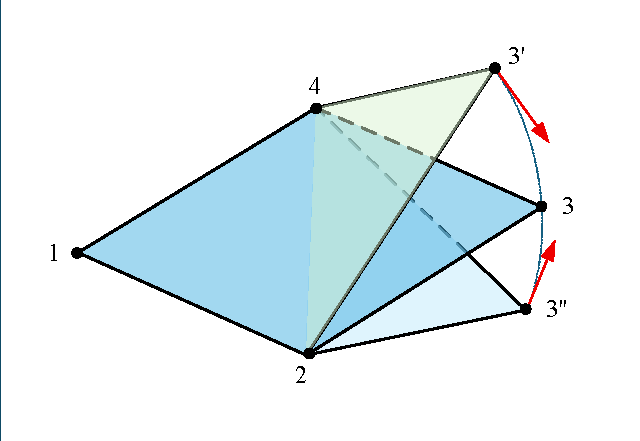
\includegraphics[width=\columnwidth,trim=2pt 2pt 2pt 2pt,clip]{figures/fig_4}
\caption{Coplanarity control action.}
\label{fig:coplanar_action}
\end{figure}

\begin{figure}[!t]
\centering
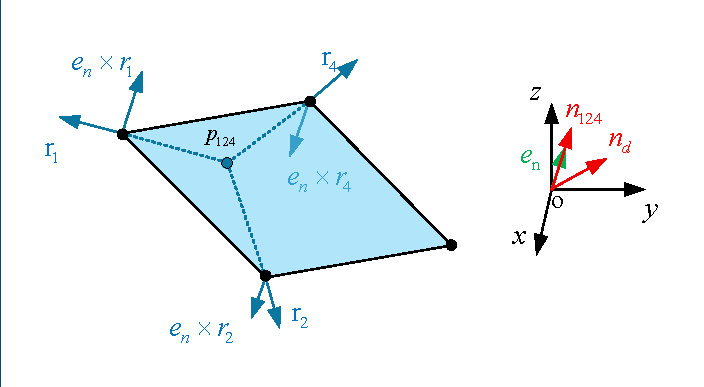
\includegraphics[width=\columnwidth,trim=2pt 2pt 2pt 2pt,clip]{figures/fig_5}
\caption{Normal-direction control action.}
\label{fig:normal_control}
\end{figure}

\subsection{QUAV Capture-Net Formation}
\label{sec:quadrotor-application}

This subsection outlines how the proposed geometric formation controller can be embedded into a QUAV-based capture-net system. As illustrated in Fig.~\ref{fig:cable_square_measurements}, the four QUAVs carry an elastic net while the formation layer uses local geometric measurements to generate the desired translational accelerations. The simplified QUAV dynamics are first introduced, then the elastic cable force and the resulting lumped disturbances are included, and finally an LESO-based compensation law is used to recover the nominal acceleration command.
\begin{figure}[!t]
\centering
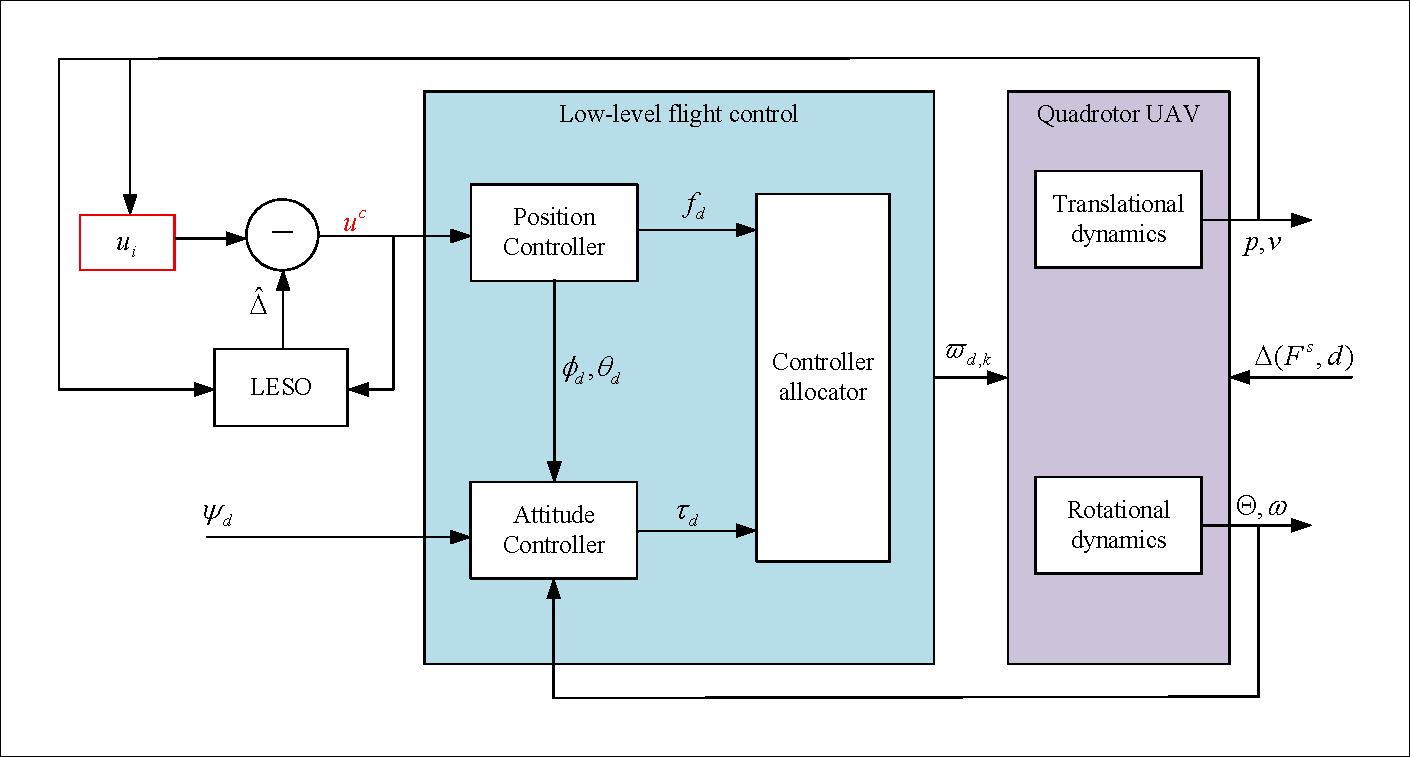
\includegraphics[width=0.85\columnwidth,trim=2pt 2pt 2pt 2pt,clip]{figures/fig_6}
\caption{Cable-connected square formation with local measurements. Red: distance measurements (\(d_{12},d_{14}\)); blue: bearing measurements. Solid lines: capture-net cables.}
\label{fig:cable_square_measurements}
\end{figure}

Following the simplified QUAV model used in \cite{li2025localInfo}, the low-level controller is separated into a position loop and an attitude loop. Let \(p_i=[p_{h,i}^T,p_{z,i}]^T\), where \(p_{h,i}=[p_{x,i},p_{y,i}]^T\in\mathbb R^2\) is the horizontal position and \(p_{z,i}\in\mathbb R\) is the altitude. The corresponding velocities are denoted by \(v_{h,i}\) and \(v_{z,i}\). The nominal horizontal channel is
\begin{equation}
\begin{aligned}
\dot p_{h,i}&=v_{h,i},\\
\dot v_{h,i}&=-gA_{\psi_i}\Theta_{h,i},
\end{aligned}
\label{eq:quadrotor-nominal-horizontal}
\end{equation}
and the nominal altitude channel is
\begin{equation}
\begin{aligned}
\dot p_{z,i}&=v_{z,i},\\
\dot v_{z,i}&=g-\frac{f_i}{m_i}.
\end{aligned}
\label{eq:quadrotor-nominal-altitude}
\end{equation}
Here, \(g\in\mathbb R\) is the gravitational constant, \(f_i\in\mathbb R\) is the total thrust, \(m_i\in\mathbb R\) is the QUAV mass, and \(\phi_i\in(-\pi/2,\pi/2)\), \(\theta_i\in(-\pi/2,\pi/2)\), and \(\psi_i\in(-\pi,\pi)\) denote the roll, pitch, and yaw angles, respectively. Moreover,
\begin{equation}
\begin{aligned}
A_{\psi_i}&=R_{\psi_i}
\begin{bmatrix}
0&1\\
-1&0
\end{bmatrix},\qquad
\Theta_{h,i}=
\begin{bmatrix}
\phi_i\\
\theta_i
\end{bmatrix},\\
R_{\psi_i}&=
\begin{bmatrix}
\cos\psi_i&-\sin\psi_i\\
\sin\psi_i&\cos\psi_i
\end{bmatrix}.
\end{aligned}
\label{eq:horizontal-attitude-map}
\end{equation}
The capture net is modeled as a set of massless elastic cables connecting selected QUAV pairs. Let \(\mathcal E_s\) denote the cable graph and \(l_{ij}^0\) the rest length of cable \((i,j)\in\mathcal E_s\). A unilateral spring-damper approximation gives the tension magnitude
\begin{equation}
T_{ij}=
\begin{cases}
k_s(d_{ij}-l_{ij}^0)+c_s\dot d_{ij}, & d_{ij}>l_{ij}^0,\\
0, & d_{ij}\le l_{ij}^0,
\end{cases}
\label{eq:cable-tension}
\end{equation}
where \(k_s>0\) and \(c_s>0\) are the cable stiffness and damping coefficients. The resultant cable force on QUAV \(i\) is
\begin{equation}
F_i^{s}=\sum_{j\in\mathcal N_i^s}T_{ij}b_{ij},
\label{eq:cable-force}
\end{equation}
where \(\mathcal N_i^s=\{j\mid (i,j)\in\mathcal E_s\}\).

The translational dynamics are subject to external disturbances such as aerodynamic drag and wind gusts, system uncertainties including modeling errors and unmodeled dynamics, residual errors from attitude tracking and thrust allocation, and cable-induced forces from the capture net. Let \(d_i^{\rm ext}\), \(\delta_i^{\rm sys}\), and \(\varepsilon_i\) denote the external disturbance, system uncertainty, and actuation residual, respectively. The lumped disturbance is defined as
\begin{equation}
\Delta_i=d_i^{\rm ext}+\delta_i^{\rm sys}+\varepsilon_i+\frac{1}{m_i}F_i^s,
\label{eq:lumped-disturbance}
\end{equation}
where \(F_i^s\) is the cable force given in~\eqref{eq:cable-force}. Its horizontal and vertical components are \(\Delta_{h,i}=S_h\Delta_i\) and \(\Delta_{z,i}=S_z\Delta_i\), with \(S_h=[I_2\;0_{2\times1}]\) and \(S_z=[0_{1\times2}\;1]\).

\begin{assumption}
\label{ass:disturbance-bounded}
The lumped disturbance \(\Delta_i\) and its derivative \(\dot\Delta_i\) are bounded, i.e., there exist positive constants \(\Delta_{i0}\) and \(\bar\Delta_{i0}\) such that \(\|\Delta_i(t)\|<\Delta_{i0}\) and \(\|\dot\Delta_i(t)\|<\bar\Delta_{i0}\) for all \(t\ge0\).
\end{assumption}

The actual translational dynamics of QUAV \(i\) are then
\begin{equation}
\begin{aligned}
\dot p_{h,i}&=v_{h,i},\\
\dot v_{h,i}&=-gA_{\psi_i}\Theta_{h,i}+\Delta_{h,i},
\end{aligned}
\label{eq:quadrotor-horizontal}
\end{equation}
and
\begin{equation}
\begin{aligned}
\dot p_{z,i}&=v_{z,i},\\
\dot v_{z,i}&=g-\frac{f_i}{m_i}+\Delta_{z,i}.
\end{aligned}
\label{eq:quadrotor-altitude}
\end{equation}

To compensate for the lumped disturbance, the formation controller~\eqref{eq:total-control} provides the nominal acceleration command \(u_i\), and the LESO supplies the disturbance estimate \(\hat\Delta_i\). The compensated acceleration command is
\begin{equation}
u_i^c=u_i-\hat\Delta_i.
\label{eq:compensated-outer-command}
\end{equation}

For each QUAV \(i\in\mathcal V\) and each coordinate axis \(\sigma\in\{x,y,z\}\), define
\begin{equation}
x_{1,i\sigma}=p_{i\sigma},\qquad
x_{2,i\sigma}=v_{i\sigma},\qquad
y_{i\sigma}=p_{i\sigma}.
\label{eq:leso-state-definition}
\end{equation}
Let \(u_{i\sigma}^c\) denote the \(\sigma\)-axis component of \(u_i^c\). For LESO design, the per-axis translational channel is written as
\begin{equation}
\begin{aligned}
\dot x_{1,i\sigma}&=x_{2,i\sigma},\\
\dot x_{2,i\sigma}&=u_{i\sigma}^c+\Delta_{i\sigma},\\
y_{i\sigma}&=x_{1,i\sigma},
\end{aligned}
\label{eq:leso-plant-form}
\end{equation}
where \(\Delta_{i\sigma}\) is the \(\sigma\)-axis component of the lumped disturbance \(\Delta_i\) defined in~\eqref{eq:lumped-disturbance}. Treating \(\Delta_{i\sigma}\) as an extended state, i.e., \(x_{3,i\sigma}=\Delta_{i\sigma}\), the LESO is designed as
\begin{equation}
\begin{aligned}
e_{i\sigma}&=z_{1,i\sigma}-y_{i\sigma},\\
\dot z_{1,i\sigma}&=z_{2,i\sigma}-\beta_{01}e_{i\sigma},\\
\dot z_{2,i\sigma}&=z_{3,i\sigma}+u_{i\sigma}^c-\beta_{02}e_{i\sigma},\\
\dot z_{3,i\sigma}&=-\beta_{03}e_{i\sigma},
\end{aligned}
\label{eq:leso-design}
\end{equation}
where \(z_{1,i\sigma}\), \(z_{2,i\sigma}\), and \(z_{3,i\sigma}\) estimate \(p_{i\sigma}\), \(v_{i\sigma}\), and \(\Delta_{i\sigma}\), respectively. The observer gains \(\beta_{01},\beta_{02},\beta_{03}>0\) are selected such that the observer error dynamics are sufficiently fast compared with the formation dynamics.

Stacking the disturbance estimates gives
\begin{equation}
\hat\Delta_i=
\begin{bmatrix}
z_{3,ix}&z_{3,iy}&z_{3,iz}
\end{bmatrix}^{T}.
\label{eq:leso-disturbance-stack}
\end{equation}
The compensation law \eqref{eq:compensated-outer-command} then recovers the nominal acceleration model \(\dot p_i=v_i\), \(\dot v_i=u_i\) when \(z_{3,i\sigma}\) accurately estimates \(\Delta_{i\sigma}\).

The resulting control structure of a single QUAV is illustrated in Fig.~\ref{fig:quav_control_structure}. The outer position loop implements the formation controller~\eqref{eq:total-control} with LESO-based disturbance compensation~\eqref{eq:compensated-outer-command}, while the inner attitude loop uses a PD controller to track the desired attitude commands.

The compensated acceleration command \(u_i^c\) is decomposed into horizontal and vertical components. The horizontal component is assigned to the horizontal position channel as
\begin{equation}
u_{h,i}^{d}=S_hu_i^c.
\label{eq:horizontal-command}
\end{equation}
According to \eqref{eq:quadrotor-nominal-horizontal}, the desired roll and pitch are obtained by inverting the horizontal channel:
\begin{equation}
\Theta_{h,i}^{d}=-\frac{1}{g}A_{\psi_i}^{-1}u_{h,i}^{d}.
\label{eq:roll-pitch-command}
\end{equation}
The vertical component determines the desired total thrust through
\begin{equation}
u_{z,i}^{d}=S_zu_i^c,
\qquad
f_i^{d}=m_i(g-u_{z,i}^{d}).
\label{eq:altitude-thrust-command}
\end{equation}
The desired yaw \(\psi_i^d\) is prescribed independently. The attitude PD controller tracks \(\phi_i^d\), \(\theta_i^d\), and \(\psi_i^d\), and generates the rotor speeds \(\omega_{i,k}\) (\(k=1,\ldots,4\)) through the standard QUAV allocation map.
\begin{figure}[ht]
\centering
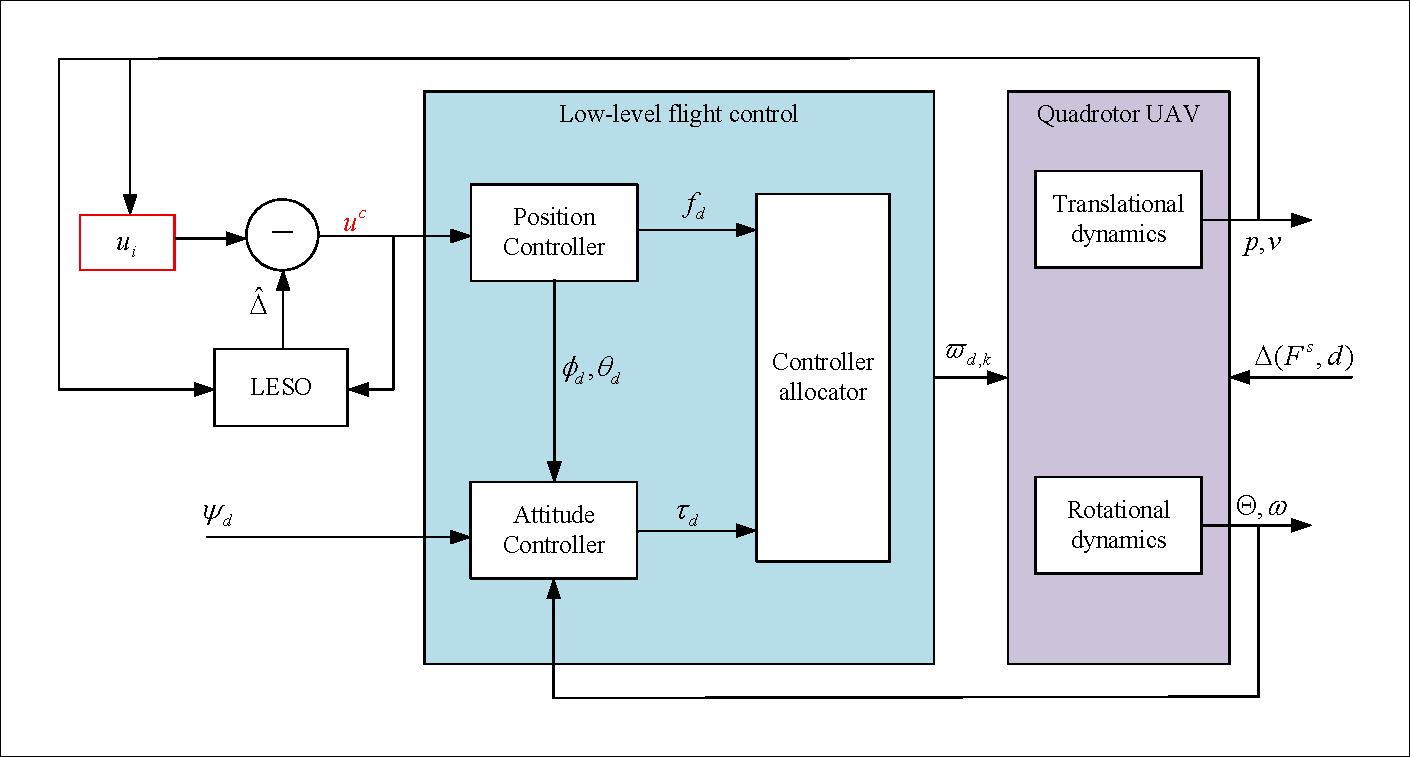
\includegraphics[width=\columnwidth,trim=2pt 2pt 2pt 2pt,clip]{figures/fig_7}
\caption{Control structure of a single QUAV.}
\label{fig:quav_control_structure}
\end{figure}

\section{Simulations}
\label{sec:simulations}

In this section, simulation results are presented to verify the effectiveness of the proposed formation control scheme. Two experiments are carried out: the first examines the coplanarity constraint using the double-integrator model~\eqref{eq:agent-dynamics}, and the second demonstrates a target capture scenario using the QUAV model with LESO-based disturbance compensation introduced in Section~\ref{sec:quadrotor-application}.

\subsection{Coplanarity Constraint Necessity}

The full controller~\eqref{eq:total-control} is compared with a reduced version where \(k_{\mathrm{cop}}=0\), using the double-integrator model~\eqref{eq:agent-dynamics} with \(n_d=[0,0,-1]^{T}\) fixed. The desired formation is a square with \(\ell^*=1.0\)~m and \(v_c^*=[0.1,0.1,0]^{T}\)~m/s. The control gains are \(k_\theta=1.67\), \(k_d=3.70\), \(k_n=4.01\), \(k_{\mathrm{cop}}=6.5\), and \(k_v=7.0\). The initial positions are chosen close to a square in the \(xy\)-plane with a deliberate out-of-plane perturbation on agent~\#3: \(p_1(0)=[0,0.6,0]^{T}\)~m, \(p_2(0)=[0,0,0]^{T}\)~m, \(p_3(0)=[0.6,0,0.05]^{T}\)~m, \(p_4(0)=[0.6,0.6,0]^{T}\)~m, and \(v_i(0)=[0,0,0]^{T}\)~m/s.

The results are shown in Figs.~\ref{fig:exp1_angle}--\ref{fig:exp1_coplanar}. Under the full controller, all angle errors converge to zero, the height of agent~\#3 returns to the reference plane, and the coplanarity error is driven to zero. With \(k_{\mathrm{cop}}=0\), a clear performance degradation is observed: agent~\#3 fails to return to the plane, its height drifting to \(0.22\)~m (Fig.~\ref{fig:exp1_height}); the coplanarity error reaches \(-0.15\) with no sign of convergence (Fig.~\ref{fig:exp1_coplanar}); and the angle errors exhibit steady-state offsets of \(10^{-2}\)~rad (Fig.~\ref{fig:exp1_angle}(b)). From the characteristic polynomial~\eqref{eq:char-poly}, \(k_{\mathrm{cop}}=0\) degenerates the coplanarity eigenvalue to zero, introducing a marginally stable mode that accounts for the observed steady-state errors. The coplanarity term is thus structurally necessary.

\begin{figure}[ht]
\centering
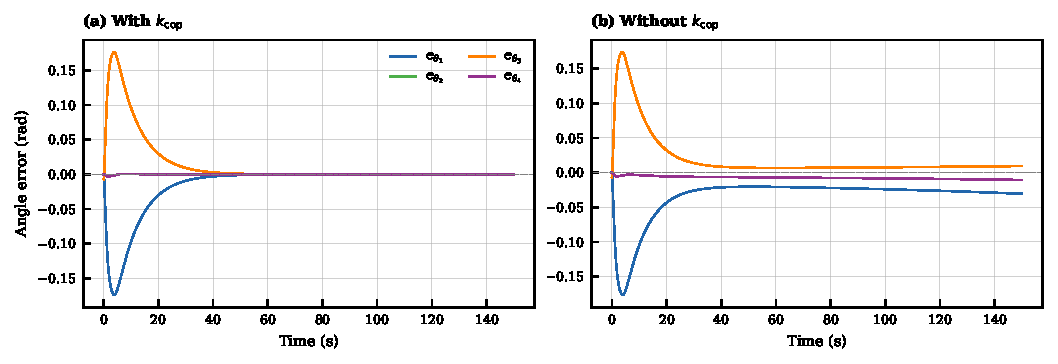
\includegraphics[width=\columnwidth,trim=2pt 2pt 2pt 2pt,clip]{figures/fig_exp1_angle}
\caption{Experiment~1: evolution of the four angle errors \(e_{\theta_1},\dots,e_{\theta_4}\). (a) Full controller with coplanarity term. (b) Controller without coplanarity term.}
\label{fig:exp1_angle}
\end{figure}

\begin{figure}[ht]
\centering
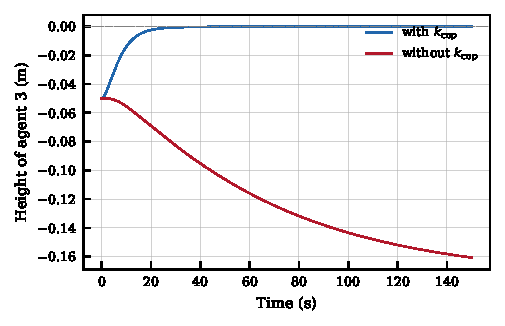
\includegraphics[width=\columnwidth,trim=2pt 2pt 2pt 2pt,clip]{figures/fig_exp1_height}
\caption{Experiment~1: height of agent~\#3 over time under the full and reduced controllers.}
\label{fig:exp1_height}
\end{figure}

\begin{figure}[ht]
\centering
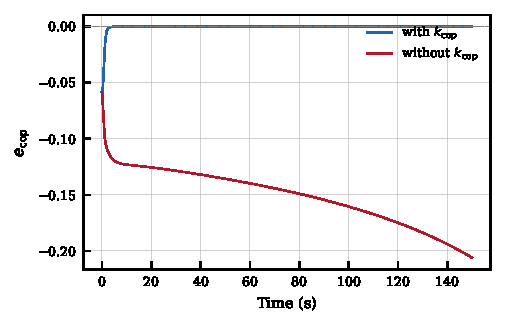
\includegraphics[width=\columnwidth,trim=2pt 2pt 2pt 2pt,clip]{figures/fig_exp1_coplanar}
\caption{Experiment~1: coplanarity error \(e_{\mathrm{cop}}\) under the full and reduced controllers.}
\label{fig:exp1_coplanar}
\end{figure}

% \FloatBarrier

\subsection{Target Capture Scenario}

The controller~\eqref{eq:total-control} is demonstrated in a target-capture task where four QUAVs carry an elastic net to intercept a moving target. The QUAV model with LESO-based disturbance compensation (Section~\ref{sec:quadrotor-application}) is adopted with \(m_i=1.5\)~kg, \(g=9.81\)~m/s\(^2\), \(I_{xx}=I_{yy}=1.745\times10^{-2}\)~kg\(\cdot\)m\(^2\), \(I_{zz}=3.175\times10^{-2}\)~kg\(\cdot\)m\(^2\), and LESO bandwidth \(\omega_o=8\)~rad/s. The control gains are \(k_\theta=3.0\), \(k_d=5.0\), \(k_n=3.5\), \(k_{\mathrm{cop}}=4.5\), and \(k_v=12.0\). The elastic cables have stiffness \(k_s=74\)~N/m, damping \(c_s=18\)~N\(\cdot\)s/m, and rest length \(l_0=1.0\)~m. The cable topology forms a closed square loop \(\mathcal{E}_s=\{(1,2),(2,3),(3,4),(4,1)\}\). The desired side length and plane normal are given by
\begin{equation}
\ell^*(t)=
\begin{cases}
1.0~\mathrm{m}, & 0\le t<60~\mathrm{s},\\[4pt]
0.4~\mathrm{m}, & t\ge 60~\mathrm{s},
\end{cases}
\label{eq:ell-star-piecewise}
\end{equation}
\begin{equation}
n_d(t)=
\begin{cases}
[1,\,0,\,0]^{T}, & 0\le t<60~\mathrm{s},\\[6pt]
[0,\,0,\,-1]^{T}, & t\ge 60~\mathrm{s}.
\end{cases}
\label{eq:nd-piecewise}
\end{equation}
The scenario proceeds in three phases:

\begin{enumerate}[leftmargin=*,nosep]
\item \emph{Net deployment} (\(0\le t<40\)~s): the formation expands from the initial compact \(0.4\)~m square toward the target formation defined by~\eqref{eq:ell-star-piecewise}--\eqref{eq:nd-piecewise}, tracking \(v_c^*=[0.1,0,0]^{T}\)~m/s.
\item \emph{Approach} (\(40\le t<50\)~s): the formation maintains the desired square shape and continues approaching the target while keeping the net plane perpendicular to the ground.
\item \emph{Target capture} (\(50\le t\le 90\)~s). At \(t=50\)~s, a smooth time-varying disturbance~\eqref{eq:pulse-disturbance} is applied. At \(t=60\)~s, the desired side length and plane normal are smoothly transitioned via tracking differentiators (TDs)~\cite{han2009PIDtoADRC} according to~\eqref{eq:ell-star-piecewise}--\eqref{eq:nd-piecewise}, driving the formation to close and orient the net plane upward for the remainder of the simulation.
\end{enumerate}

To validate the LESO-based disturbance compensation, a smooth time-varying disturbance is applied to each QUAV during \(t\in[50,60]\)~s:
\begin{equation}
\Delta_i(t)=A\sin^{2}\!\left(\pi\frac{t-50}{10}\right)\mathbf{d},\qquad t\in[50,60]~\mathrm{s},
\label{eq:pulse-disturbance}
\end{equation}
with \(A=1.0\)~N and direction \(\mathbf{d}=[-0.8,0.4,0.45]^{T}/\|\cdot\|\).

The initial positions form a compact \(0.4\)~m square: \(p_1(0)=[0,0.4,0]^{T}\)~m, \(p_2(0)=[0,0,0]^{T}\)~m, \(p_3(0)=[0.4,0,0]^{T}\)~m, \(p_4(0)=[0.4,0.4,0]^{T}\)~m, with \(v_i(0)=[0,0,0]^{T}\)~m/s.

The results are shown in Figs.~\ref{fig:exp2_leso_x}--\ref{fig:exp2_trajectory}. The formation expands from the initial compact configuration to the \(1.0\)~m square, approaches the incoming target, and closes to \(0.4\)~m after the TD-smoothed transition at \(t=60\)~s (Fig.~\ref{fig:exp2_trajectory}). All formation errors exhibit transients during the disturbance interval (\(t\in[50,60]\)~s) and the parameter switch, and then converge. The LESO accurately estimates the lumped disturbance on all three axes for every QUAV, enabling the formation to maintain satisfactory tracking performance throughout the maneuver (Figs.~\ref{fig:exp2_leso_x}--\ref{fig:exp2_leso_z}).

\begin{figure}[ht]
\centering
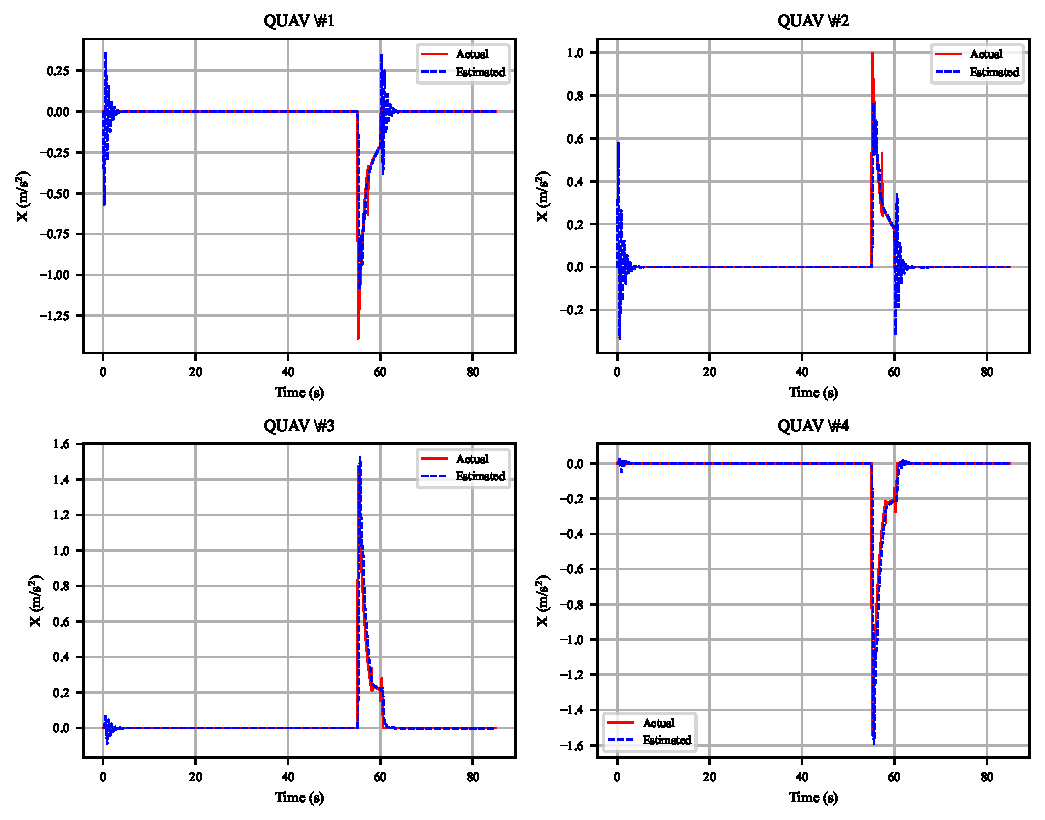
\includegraphics[width=\columnwidth,trim=2pt 2pt 2pt 2pt,clip]{figures/fig_exp2_leso_x}
\caption{Experiment~2: LESO disturbance estimation on the \(x\)-axis. Actual (red) and estimated (blue dashed) lumped disturbance accelerations for all four QUAVs.}
\label{fig:exp2_leso_x}
\end{figure}

\begin{figure}[ht]
\centering
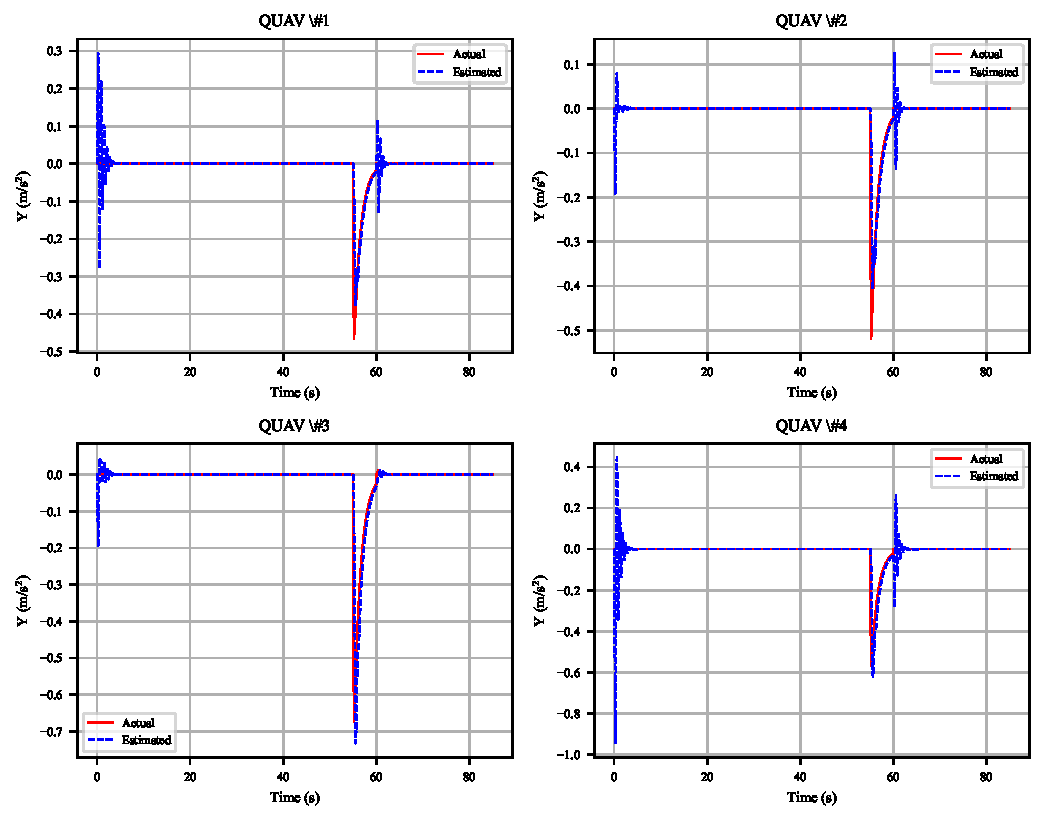
\includegraphics[width=\columnwidth,trim=2pt 2pt 2pt 2pt,clip]{figures/fig_exp2_leso_y}
\caption{Experiment~2: LESO disturbance estimation on the \(y\)-axis.}
\label{fig:exp2_leso_y}
\end{figure}

\begin{figure}[ht]
\centering
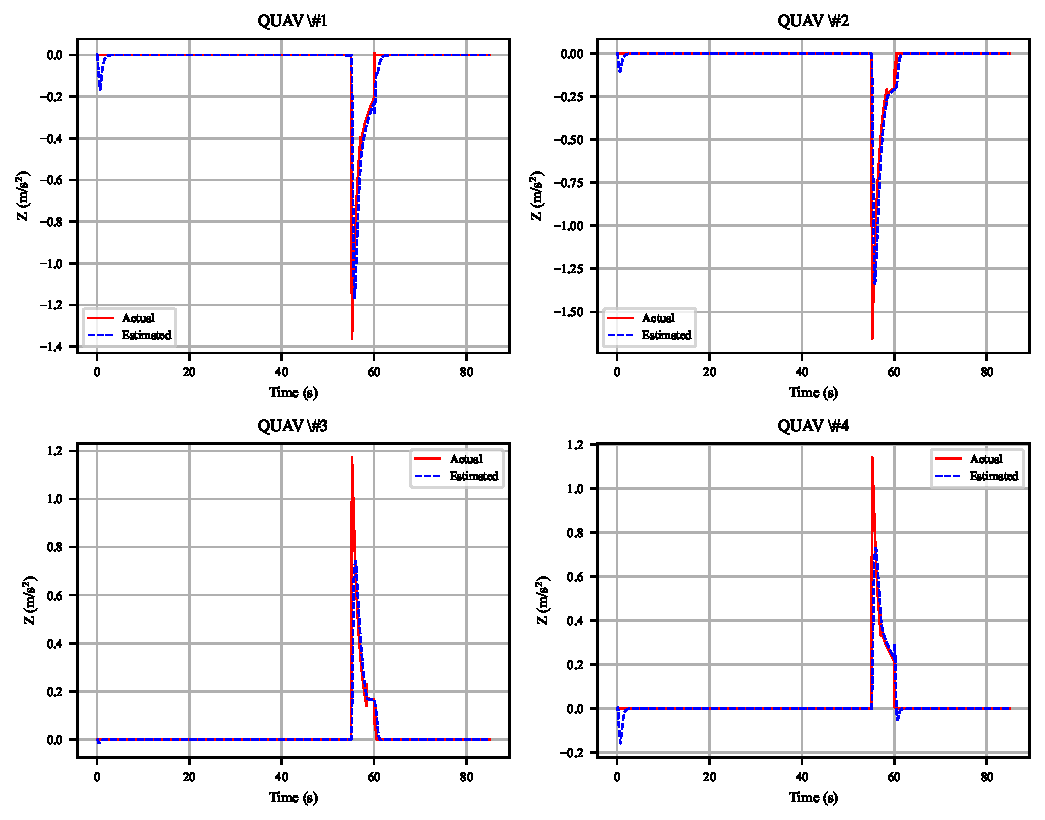
\includegraphics[width=\columnwidth,trim=2pt 2pt 2pt 2pt,clip]{figures/fig_exp2_leso_z}
\caption{Experiment~2: LESO disturbance estimation on the \(z\)-axis.}
\label{fig:exp2_leso_z}
\end{figure}

\begin{figure}[t]
\centering
\subfloat[Angle errors \(e_{\theta_i}\)]{
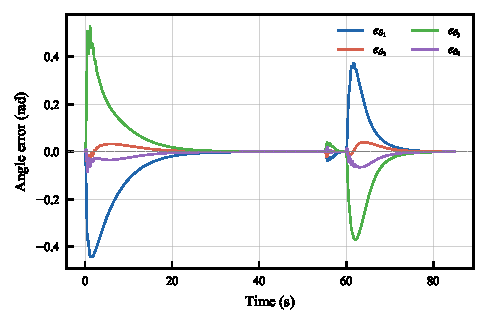
\includegraphics[width=0.44\columnwidth,trim=2pt 2pt 2pt 2pt,clip]{figures/fig_exp2_angle}
\label{fig:exp2_angle}}
\hspace{4pt}
\subfloat[Edge distances \(d_{ij}\)]{
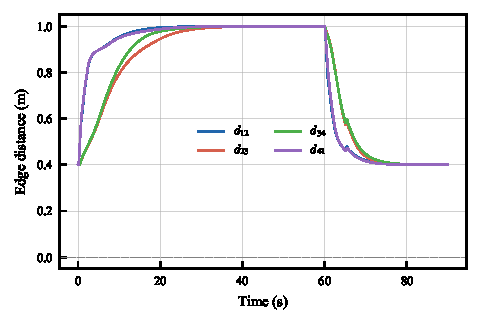
\includegraphics[width=0.44\columnwidth,trim=2pt 2pt 2pt 2pt,clip]{figures/fig_exp2_edge}
\label{fig:exp2_edge}}
\\[0pt]
\subfloat[Coplanarixty error \(e_{\mathrm{cop}}\)]{
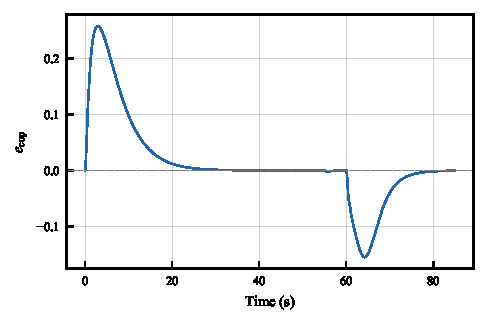
\includegraphics[width=0.44\columnwidth,trim=2pt 2pt 2pt 2pt,clip]{figures/fig_exp2_coplanar}
\label{fig:exp2_coplanar}}
\hspace{4pt}
\subfloat[Normal-direction error \(\|e_n\|\)]{
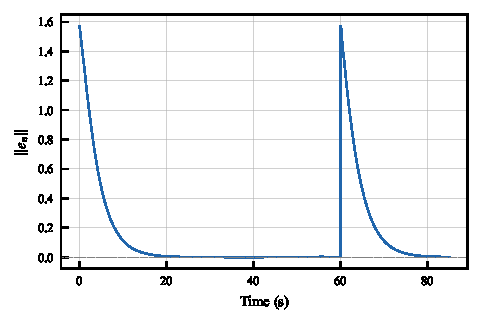
\includegraphics[width=0.44\columnwidth,trim=2pt 2pt 2pt 2pt,clip]{figures/fig_exp2_norm}
\label{fig:exp2_norm}}
\caption{Experiment~2: evolution of formation errors.}
\label{fig:exp2_errors}
\end{figure}

\begin{figure*}[t]
\centering
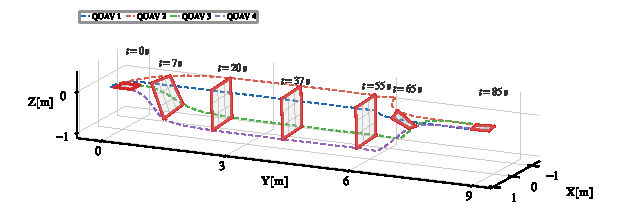
\includegraphics[width=\textwidth,trim=2pt 2pt 2pt 2pt,clip]{figures/fig_exp2_trajectory}
\caption{Experiment~2: 3-D trajectories of the four QUAVs and the target.}
\label{fig:exp2_trajectory}
\end{figure*}

\section{Conclusion}
This paper addressed the distributed formation control problem of four agents forming a planar square in 3-D space. For a concyclic square, unsigned angle and distance constraints specify the in-plane shape and scale but leave the plane orientation as a free degree of freedom in 3-D. To prescribe the orientation, an undirected plane-normal control scheme was introduced. By treating \(\pm n_d\) as equivalent target orientations and employing a hysteresis-based branch selection with a deadzone, the controller avoids both the singularity of a raw cross product formulation and the chattering problem near perpendicular configurations, while ensuring the formation plane aligns with the target plane. A coplanarity constraint was further incorporated and shown, via a perturbation analysis, to provide first-order sensitivity to out-of-plane deviations, whereas angle-based terms provide only second-order sensitivity, establishing its necessity for maintaining coplanarity. A five-term distributed controller was proposed, and local exponential stability of the nominal closed-loop system was established by constructing minimal internal error coordinates and proving Hurwitzness of the linearized system.

Future work includes experimental validation, extension to formations with more agents, analysis of the hybrid dynamics arising from branch switching, and incorporation of disturbance compensation for operation in realistic environments.

\section*{Acknowledgments}

This work was supported in part by the National Natural Science Foundation of China (Grant No. 12272116 and 12372050).

\appendices
\section{Explicit Linearized Matrices and Supplementary Calculations}

\subsection{Local error-coordinate Jacobians}
\label{app:error-jacobians}

This subsection records the Jacobians used to remove the redundant angle error \(e_{\theta_3}\). With the local coordinate \(\xi\) defined in the proof of Theorem~\ref{thm:local-stability}, the minimal error map \(\hat h(\xi)=\hat\eta\) satisfies
\begin{equation}
\resizebox{\columnwidth}{!}{$
J_{sq}=D\hat h(0)=
\begin{bmatrix}
1&0&0&0&0&0&0&0\\
0&0&0&0&0&1&0&0\\
-\frac{1}{\ell^*}&0&0&0&0&0&\frac{1}{\ell^*}&0\\
0&0&0&-\frac{1}{\ell^*}&0&0&0&0\\
\frac{1}{\ell^*}&0&\frac{1}{\ell^*}&0&0&-\frac{1}{\ell^*}&-\frac{1}{\ell^*}&0\\
0&-\frac{\sqrt2}{2\ell^*}&0&0&-\frac{\sqrt2}{2\ell^*}&0&0&\frac{\sqrt2}{2\ell^*}\\
0&-\frac{1}{\ell^*}&0&0&0&0&0&0\\
0&-\frac{1}{\ell^*}&0&0&0&0&0&\frac{1}{\ell^*}
\end{bmatrix}.
$}
\label{eq:Jsq}
\end{equation}
Since \(\det J_{sq}=-\sqrt2/(2(\ell^*)^6)\neq0\), the minimal error vector is a valid local coordinate.

For the raw error map \(h_{\mathrm{raw}}(\xi)=\eta^{\mathrm{raw}}\), the Jacobian is
\begin{equation}
\resizebox{\columnwidth}{!}{$
J_{\mathrm{raw}}=Dh_{\mathrm{raw}}(0)=
\begin{bmatrix}
1&0&0&0&0&0&0&0\\
0&0&0&0&0&1&0&0\\
-\frac{1}{\ell^*}&0&0&0&0&0&\frac{1}{\ell^*}&0\\
0&0&0&-\frac{1}{\ell^*}&0&0&0&0\\
0&0&-\frac{1}{\ell^*}&\frac{1}{\ell^*}&0&\frac{1}{\ell^*}&0&0\\
\frac{1}{\ell^*}&0&\frac{1}{\ell^*}&0&0&-\frac{1}{\ell^*}&-\frac{1}{\ell^*}&0\\
0&-\frac{\sqrt2}{2\ell^*}&0&0&-\frac{\sqrt2}{2\ell^*}&0&0&\frac{\sqrt2}{2\ell^*}\\
0&-\frac{1}{\ell^*}&0&0&0&0&0&0\\
0&-\frac{1}{\ell^*}&0&0&0&0&0&\frac{1}{\ell^*}
\end{bmatrix}.
$}
\label{eq:Jraw}
\end{equation}
The fifth row, corresponding to \(e_{\theta_3}\), satisfies
\begin{equation}
J_{\mathrm{raw}}^{(5)}+J_{\mathrm{raw}}^{(3)}
+J_{\mathrm{raw}}^{(4)}+J_{\mathrm{raw}}^{(6)}=0.
\label{eq:Jraw-row-relation}
\end{equation}
Thus, to first order, \(e_{\theta_3}=-(e_{\theta_1}+e_{\theta_2}+e_{\theta_4})\). This row relation gives the embedding matrix \(S=Dg(0)\) in \eqref{eq:S-matrix}, while the matrix \(R\) in \eqref{eq:Astar} simply removes the fifth row of \(\eta^{\mathrm{raw}}\).

\subsection{The matrix \(C^*\)}
\label{app:Cstar}

At the target square \eqref{eq:target-square} with the bearing vectors \eqref{eq:target-bearings}, the linearized kinematic matrix \(C^*\in\mathbb R^{9\times 12}\) relating \(\dot\eta=C^*\tilde v\) has the following rows. We use the compact notation where each row is partitioned as \([c_1\,|\,c_2\,|\,c_3\,|\,c_4]\) with \(c_i\in\mathbb R^{1\times 3}\) being the coefficient row for \(\tilde v_i\).

\noindent\textbf{Rows 1--2 (distance errors):}
\begin{align}
\dot e_{12}&=[0,1,0\;|\;0,-1,0\;|\;0,0,0\;|\;0,0,0]\,\tilde v,\\
\dot e_{14}&=[-1,0,0\;|\;0,0,0\;|\;0,0,0\;|\;1,0,0]\,\tilde v.\notag
\end{align}

\noindent\textbf{Rows 3--6 (angle errors):} From \eqref{eq:alphadot} evaluated at the target (\(\sin\alpha_i^*=1\), all adjacent edges of length \(\ell^*\)):
\begin{align}
\dot e_{\theta_1}&=\frac{1}{\ell^*}[1,-1,0\;|\;-1,0,0\;|\;0,0,0\;|\;0,1,0]\,\tilde v,\\
\dot e_{\theta_2}&=\frac{1}{\ell^*}[-1,0,0\;|\;1,1,0\;|\;0,-1,0\;|\;0,0,0]\,\tilde v,\notag\\
\dot e_{\theta_3}&=\frac{1}{\ell^*}[0,0,0\;|\;0,-1,0\;|\;-1,1,0\;|\;1,0,0]\,\tilde v,\notag\\
\dot e_{\theta_4}&=\frac{1}{\ell^*}[0,1,0\;|\;0,0,0\;|\;1,0,0\;|\;-1,-1,0]\,\tilde v.\notag
\end{align}

\noindent\textbf{Row 7 (coplanarity error):}
\begin{equation}
\dot e_{\mathrm{cop}}=\frac{1}{\sqrt2\,\ell^*}[0,0,-1\;|\;0,0,1\;|\;0,0,-1\;|\;0,0,1]\,\tilde v.
\end{equation}

\noindent\textbf{Rows 8--9 (normal error components):}
\begin{align}
(\dot e_n^\perp)_1&=\frac{1}{\ell^*}[0,0,-1\;|\;0,0,1\;|\;0,0,0\;|\;0,0,0]\,\tilde v,\\
(\dot e_n^\perp)_2&=\frac{1}{\ell^*}[0,0,-1\;|\;0,0,0\;|\;0,0,0\;|\;0,0,1]\,\tilde v.\notag
\end{align}

Observe that rows 1--6 depend only on the in-plane components of \(\tilde v\), whereas rows 7--9 depend only on the out-of-plane components. This structural decoupling is fundamental to the factorization of the characteristic polynomial.

\subsection{The matrix \(-B^*\)}
\label{app:Bstar}

The linearized control matrix \(-B^*\in\mathbb R^{12\times 9}\) encodes the acceleration response to each geometric error. We present it column by column; each column is a \(12\times 1\) vector partitioned as \([a_1\,|\,a_2\,|\,a_3\,|\,a_4]^{T}\) where \(a_i\in\mathbb R^{3}\) is the acceleration on agent~\(i\).

\noindent\textbf{Columns 1--2 (distance errors \(e_{12},e_{14}\)):}
\begin{align}
\mathrm{col}(e_{12})&=k_d\,[0,-1,0\;|\;0,1,0\;|\;0,0,0\;|\;0,0,0]^{T},\\
\mathrm{col}(e_{14})&=k_d\,[1,0,0\;|\;0,0,0\;|\;0,0,0\;|\;-1,0,0]^{T}.\notag
\end{align}

\noindent\textbf{Columns 3--6 (angle errors \(e_{\theta_1},\dots,e_{\theta_4}\)):}
\begin{align}
\mathrm{col}(e_{\theta_1})&=-k_\theta\,[1,-1,0\;|\;0,0,0\;|\;0,0,0\;|\;0,0,0]^{T},\\
\mathrm{col}(e_{\theta_2})&=-k_\theta\,[0,0,0\;|\;1,1,0\;|\;0,0,0\;|\;0,0,0]^{T},\notag\\
\mathrm{col}(e_{\theta_3})&=-k_\theta\,[0,0,0\;|\;0,0,0\;|\;-1,1,0\;|\;0,0,0]^{T},\notag\\
\mathrm{col}(e_{\theta_4})&=-k_\theta\,[0,0,0\;|\;0,0,0\;|\;0,0,0\;|\;-1,-1,0]^{T}.\notag
\end{align}

\noindent\textbf{Column 7 (coplanarity error):}
\begin{equation}
\mathrm{col}(e_{\mathrm{cop}})=k_{\mathrm{cop}}\,[0,0,0\;|\;0,0,0\;|\;0,0,1\;|\;0,0,0]^{T}.
\end{equation}

\noindent\textbf{Columns 8--9 (normal error components):} At the target square, the centroid of \(\{1,2,4\}\) is \((\ell^*/3,2\ell^*/3,0)\) and the relative position vectors are \(r_1^*=[-\ell^*/3,\ell^*/3,0]^{T}\), \(r_2^*=[-\ell^*/3,-2\ell^*/3,0]^{T}\), \(r_4^*=[2\ell^*/3,\ell^*/3,0]^{T}\). From \(u_i^{\mathrm{nor}}=k_n(e_n\times r_i)\) with \(e_n=[(e_n^\perp)_1,(e_n^\perp)_2,0]^{T}\) and \(r_{i,z}^*=0\), only the \(z\)-components are non-zero:
\begin{align}
\mathrm{col}((e_n^\perp)_1)&=\frac{k_n\ell^*}{3}\,[0,0,1\;|\;0,0,-2\;|\;0,0,0\;|\;0,0,1]^{T},\\
\mathrm{col}((e_n^\perp)_2)&=\frac{k_n\ell^*}{3}\,[0,0,1\;|\;0,0,1\;|\;0,0,0\;|\;0,0,-2]^{T}.\notag
\end{align}

Again, columns 1--6 generate only in-plane forces, while columns 7--9 generate only out-of-plane forces.

\subsection{Computation of \(\hat G^*\) and its characteristic polynomial}
\label{app:Gstar}

The minimal structure matrix is \(\hat G^*=R C^*(-B^*)S\), where \(R\) removes the row corresponding to \(e_{\theta_3}\) and \(S\) is given in \eqref{eq:S-matrix}. Direct multiplication gives
\begin{equation}
\resizebox{\columnwidth}{!}{$
\hat G^*=
\begin{bmatrix}
-2k_d&0&k_\theta&k_\theta&0&0&0&0\\
0&-2k_d&k_\theta&0&k_\theta&0&0&0\\
\frac{k_d}{\ell^*}&\frac{k_d}{\ell^*}&-\frac{2k_\theta}{\ell^*}&\frac{k_\theta}{\ell^*}&\frac{k_\theta}{\ell^*}&0&0&0\\
\frac{k_d}{\ell^*}&-\frac{k_d}{\ell^*}&0&-\frac{3k_\theta}{\ell^*}&-\frac{k_\theta}{\ell^*}&0&0&0\\
-\frac{k_d}{\ell^*}&\frac{k_d}{\ell^*}&0&-\frac{k_\theta}{\ell^*}&-\frac{3k_\theta}{\ell^*}&0&0&0\\
0&0&0&0&0&-\frac{\sqrt2}{2\ell^*}k_{\mathrm{cop}}&-\frac{\sqrt2}{3}k_n&-\frac{\sqrt2}{3}k_n\\
0&0&0&0&0&0&-k_n&0\\
0&0&0&0&0&0&0&-k_n
\end{bmatrix}.
$}
\end{equation}

The \(xy\)- and \(z\)-channels are block upper triangular. The out-of-plane diagonal entries contribute
\[
(\lambda+k_n)^2\left(\lambda+\frac{\sqrt2}{2\ell^*}k_{\mathrm{cop}}\right).
\]
For the in-plane block, direct computation gives
\[
\left(\lambda+\frac{4k_\theta}{\ell^*}\right)
\left(\lambda^2+\frac{2(k_d\ell^*+k_\theta)}{\ell^*}\lambda+\frac{2k_d k_\theta}{\ell^*}\right)^2.
\]
Multiplying these factors yields \eqref{eq:char-poly}.

\begin{thebibliography}{1}
\bibitem{rothe2019concept}
J.~Rothe, M.~Strohmeier, and S.~Montenegro, ``A concept for catching drones with a net carried by cooperative UAVs,'' in \textit{Proc. IEEE Int. Symp. Safety, Security, Rescue Robot. (SSRR)}, W\"{u}rzburg, Germany, Sep. 2019, pp. 126--132, doi: 10.1109/SSRR.2019.8848971.

\bibitem{tolman2017counter}
S.~Tolman and R.~W.~Beard, ``Counter UAS using a formation controlled dragnet,'' in \textit{Proc. Int. Conf. Unmanned Aircr. Syst. (ICUAS)}, Miami, FL, USA, Jun. 2017, pp. 1665--1672, doi: 10.1109/ICUAS.2017.7991391.

\bibitem{chakravarthy2021interception}
A.~Chakravarthy and D.~Ghose, ``Interception of intruder UAV swarms with a net manipulated by a team of UAVs,'' in \textit{Proc. AIAA Scitech Forum}, Virtual Event, Jan. 2021, Art. no. 2021-1767, doi: 10.2514/6.2021-1767.

\bibitem{wang2022discrete}
J.~Wang, L.~Zhao, and K.~Xia, ``A discrete-time intercepting strategy for net capture using multiple unmanned aerial vehicles,'' in \textit{Proc. IEEE Int. Conf. Unmanned Syst. (ICUS)}, Guangzhou, China, Oct. 2022, pp. 134--139, doi: 10.1109/ICUS55513.2022.9986777.

\bibitem{oh2015survey}
K.-K.~Oh, M.-C.~Park, and H.-S.~Ahn, ``A survey of multi-agent formation control,'' \textit{Automatica}, vol.~53, pp.~424--440, Mar. 2015, doi: 10.1016/j.automatica.2014.10.022.

\bibitem{nguyen2020gps}
T.~D.~Nguyen, ``Evaluation of the accuracy of the ship location determined by GPS global positioning system on a given sea area,'' \textit{J. Phys. Conf. Ser.}, vol.~1515, no.~4, 2020, Art. no.~042010.

\bibitem{demarina2021displacement}
H.~G.~de~Marina, ``Maneuvering and robustness issues in undirected displacement-consensus-based formation control,'' \textit{IEEE Trans. Autom. Control}, vol.~66, no.~7, pp.~3370--3377, Jul. 2021.

\bibitem{trinh2016bearing}
M.~H.~Trinh, G.-H.~Ko, V.~H.~Pham, K.-K.~Oh, and H.-S.~Ahn, ``Guidance using bearing-only measurements with three beacons in the plane,'' \textit{Control Eng. Pract.}, vol.~51, pp.~81--91, 2016.

\bibitem{li2025localInfo}
J.~Li, L.~Chen, and C.~Li, ``Multi-agent distributed formation control using local information measurements,'' \textit{Sci. China Technol. Sci.}, vol.~68, no.~7, Art. no.~1720402, 2025, doi: 10.1007/s11431-024-2896-5.

\bibitem{hu2023angle}
R.~Hu, X.~Huang, and C.~Xu, ``Integrated visual navigation based on angles-only measurements for asteroid final landing phase,'' \textit{Astrodynamics}, vol.~7, pp.~69--82, 2023.

\bibitem{gong2023review}
B.~Gong, S.~Wang, S.~Li, et al., ``Review of space relative navigation based on angles-only measurements,'' \textit{Astrodynamics}, vol.~7, pp.~131--152, 2023.

\bibitem{shao2024directed}
Z.~Shao, Z.~Zhou, Y.~Wang, and Y.~Song, ``Directed formation control using distance and angle in local coordinate frameworks,'' \textit{IEEE Trans. Ind. Electron.}, vol.~71, no.~11, pp.~14722--14729, Nov. 2024, doi: 10.1109/TIE.2024.3363778.

\bibitem{sun2017distributed}
Z.~Sun, M.-C.~Park, B.~D.~O.~Anderson, and H.-S.~Ahn, ``Distributed stabilization control of rigid formations with prescribed orientation,'' \textit{Automatica}, vol.~78, pp.~250--257, Apr. 2017, doi: 10.1016/j.automatica.2016.12.031.

\bibitem{li2024circle}
S.~Li, C.~Wang, and G.~Xie, ``3D circle formation control of VTOL vehicles without distance measurement,'' \textit{IEEE Trans. Intell. Veh.}, vol.~9, no.~2, pp.~3305--3315, Feb. 2024, doi: 10.1109/TIV.2023.3340875.

\bibitem{chen2022maneuvering}
L.~Chen, Z.~Lin, H.~Garcia~de~Marina, Z.~Sun, and M.~Feroskhan, ``Maneuvering angle rigid formations with global convergence guarantees,'' \textit{IEEE/CAA J. Autom. Sinica}, vol.~9, no.~8, pp.~1464--1475, Aug. 2022, doi: 10.1109/JAS.2022.105749.

\bibitem{chen2020affine}
L.~Chen, J.~Mei, C.~Li, and G.~Ma, ``Distributed leader--follower affine formation maneuver control for high-order multiagent systems,'' \textit{IEEE Trans. Autom. Control}, vol.~65, no.~11, pp.~4941--4948, Nov. 2020, doi: 10.1109/TAC.2020.2986684.

\bibitem{xu2020affine}
Y.~Xu, S.~Zhao, D.~Luo, and Y.~You, ``Affine formation maneuver control of high-order multi-agent systems over directed networks,'' \textit{Automatica}, vol.~118, Art. no.~109004, Aug. 2020, doi: 10.1016/j.automatica.2020.109004.

\bibitem{chen2023angleRigidity3D}
L.~Chen and M.~Cao, ``Angle rigidity for multiagent formations in 3-D,'' \textit{IEEE Trans. Autom. Control}, vol.~68, no.~10, pp.~6130--6145, Oct. 2023, doi: 10.1109/TAC.2023.3237799.

\bibitem{han2009PIDtoADRC}
J.~Han, ``From PID to active disturbance rejection control,'' \textit{IEEE Trans. Ind. Electron.}, vol.~56, no.~3, pp.~900--906, Mar. 2009, doi: 10.1109/TIE.2008.2011621.

\bibitem{chen2021angleRigidity}
L.~Chen, M.~Cao, and C.~Li, ``Angle rigidity and its usage to stabilize multiagent formations in 2-D,'' \textit{IEEE Trans. Autom. Control}, vol.~66, no.~8, pp.~3667--3681, Aug. 2021, doi: 10.1109/TAC.2020.3025539.

\bibitem{chen2022stabilizing}
L. Chen, Q. Yang, M. Shi, Y. Li, and M. Feroskhan, ``Stabilizing angle rigid formations with prescribed orientation and scale,'' \textit{IEEE Trans. Ind. Electron.}, vol. 69, no. 11, pp. 11654--11665, Nov. 2022, doi: 10.1109/TIE.2021.3120476.

\bibitem{chen2023angleConstrained}
L. Chen, J. Xiao, R. C. H. Lin, and M. Feroskhan, ``Angle-constrained formation maneuvering of unmanned aerial vehicles,'' \textit{IEEE Trans. Control Syst. Technol.}, vol. 31, no. 4, pp. 1733--1746, Jul. 2023, doi: 10.1109/TCST.2023.3240286.

\bibitem{wang2025esoMultiUAV}
R. Wang, T. Mei, W. Ma, and W. Hao, ``Disturbance rejection control for multi-UAV formations based extended state observer,'' in \textit{Proc. 40th Youth Acad. Annu. Conf. Chin. Assoc. Autom.}, 2025, pp. 2144--2149, doi: 10.1109/YAC66630.2025.11150314.

\bibitem{ren2026observer}
W. Ren, G.-R. Duan, P. Li, and H. Kong, ``Observer-based active fault/disturbance compensation control for fully actuated systems,'' \textit{Sci. China Inf. Sci.}, vol. 69, no. 5, Art. no. 152202, 2026, doi: 10.1007/s11432-025-4817-2.

\bibitem{khalil2002nonlinear}
H.~K.~Khalil, \textit{Nonlinear Systems}, 3rd~ed.\hfill Upper Saddle River, NJ, USA:\hfill Prentice-Hall, 2002.

\end{thebibliography}

\end{document}

